   The CLAS12 detector is a large angle spectrometer that generally covers angles from 5 to 130 degrees, spanned by two main detector subsystems - the Forward Detector and the Central Detector.

    Overview of Jefferson Lab
    Why is CLAS12 particularly suited for this measurement?

\section{Accelerator and Beamline}
    The Thomas Jefferson National Accelerator Facility, also called Jefferson Lab (JLab), is one of the 17 National Laboratories in the United States \parencite{DepartmentofEnergy2023DepartmentLaboratories}, and functions mainly to deliver high energy, continuous wave (CW) electron beams to fixed-target nuclear and particle physics experiments. The facility was established in 1984 - initially named the Continuous Electron Beam Accelerator Facility (CEBAF) - and first delivered a 4 GeV electron beam on July 1 1994 to one of its three original detector halls. In 2006 efforts began to upgrade the facility to produce an electron beam up to 12 GeV in energy, which was first successfully delivered in 2015, as well as to construct a fourth detector hall for additional physics experiments\parencite{JeffersonLab2023AboutLab}. JLab is also home to a free-electron laser, capable of 10+ kW CW operation \parencite{Benson2007HighAccelerator}. 

\begin{figure}[ht]
    \centering
    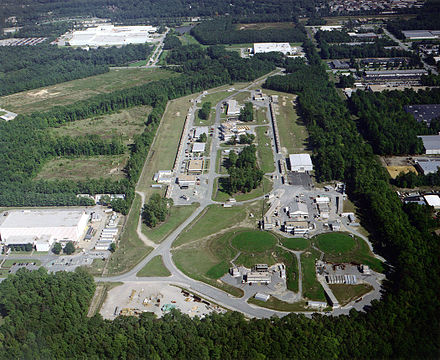
\includegraphics[width=0.8\textwidth]{Chapters/Ch2-Experiment/accel_and_beamline/pics/CEBAF/jlab_wiki.png}
    \caption{An aerial view of the Thomas Jefferson National Accelerator Facility \parencite{Wang2010CEBAFOverview}. Note that this picture was taken before the addition of the fourth detector hall (Hall D).}
    \label{fig:jlab_wiki}
\end{figure}

\subsection{Accelerator Facility}
    
    \figref{fig:jlab_accelerator_layout} shows the overarching scheme of the entire accelerator facility relevant for this experiment. Electrons are produced via the photoelectric effect from a 499 MHz pulsed laser impinges on a Gallium Arsenide photocathode (\figref{fig:gun}). The CEBAF guns operate at 100 kV and accelerate the electrons through a beam chopper (\figref{fig:chopper}) to create the desired beam structure (\figref{fig:structure}) and into the main accelerator circuit, where 1497 MHz superconducting resonator (SRF) cavities provide further acceleration (\figref{fig:klystron}). CEBAF's two $\sim$ 1.1 GV linacs accelerate electrons by consist of 50 cryomodules total, with each cryomodule housing 8 7-cell SRF cavities and the liquid helium necessary to cool them, made possible by JLab's 2K liquid helium refrigerator, the largest in the world as of 2023. The electrons are steered around the curved parts of the track by dipole magnets (\figref{fig:magnets}), making five complete circulations before delivery to the three western experimental halls.
    
    
    \begin{figure}[ht]
        \centering
        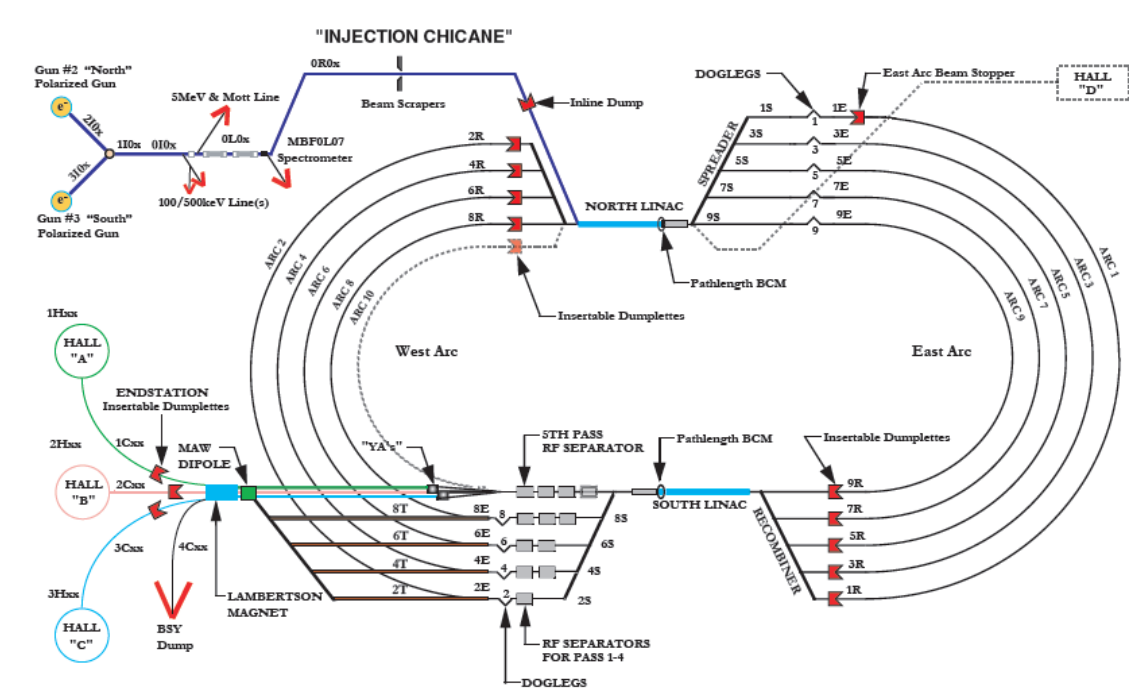
\includegraphics[width=0.8\textwidth]{Chapters/Ch2-Experiment/accel_and_beamline/pics/CEBAF/jlab-accelerator-layout.png}
        \caption{Schematic layout of the CEBAF accelerator at JLab. The racetrack configuration has two linear accelerator portions $\sim$ 1/4 mile long, and is $\sim$ 7/8 mile around \parencite{Wang2010CEBAFOverview}.}
        \label{fig:jlab_accelerator_layout}
    \end{figure}
    
    
    \begin{figure}[htb]
        \begin{minipage}[c]{\linewidth}
            \centering
            \subfloat[]{\label{fig:gun}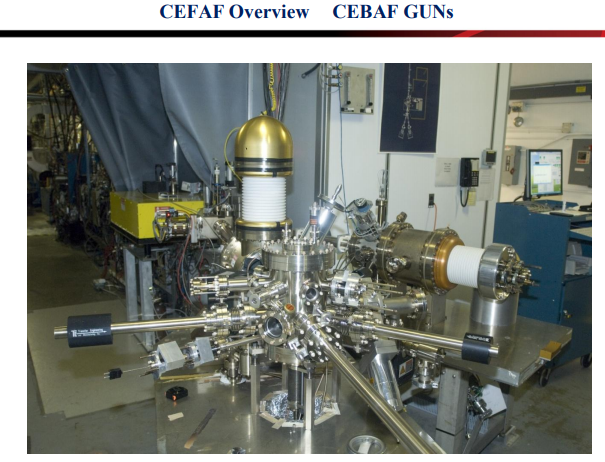
\includegraphics[width=0.3\textwidth]{Chapters/Ch2-Experiment/accel_and_beamline/pics/CEBAF/1_CEBAF-guns.png}}
            \subfloat[]{\label{fig:chopper}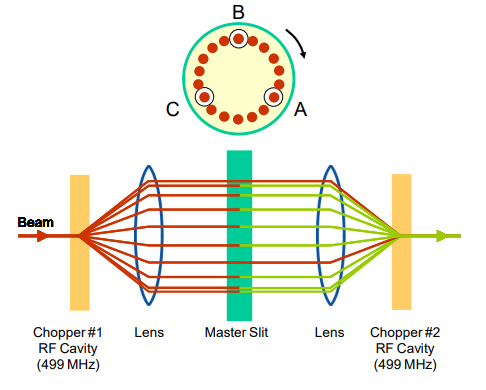
\includegraphics[width=0.3\textwidth]{Chapters/Ch2-Experiment/accel_and_beamline/pics/CEBAF/jlab-chopper.png}}
            \subfloat[]{\label{fig:structure}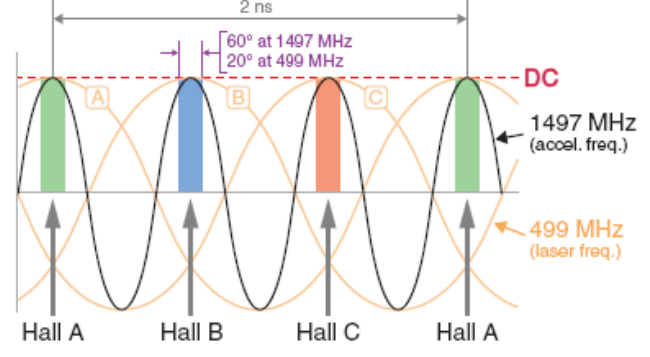
\includegraphics[width=0.3\textwidth]{Chapters/Ch2-Experiment/accel_and_beamline/pics/CEBAF/Jlab-beam-structure.png}}
        \end{minipage}
        \begin{minipage}[c]{\linewidth}
            \centering
            \subfloat[]{\label{fig:klystron}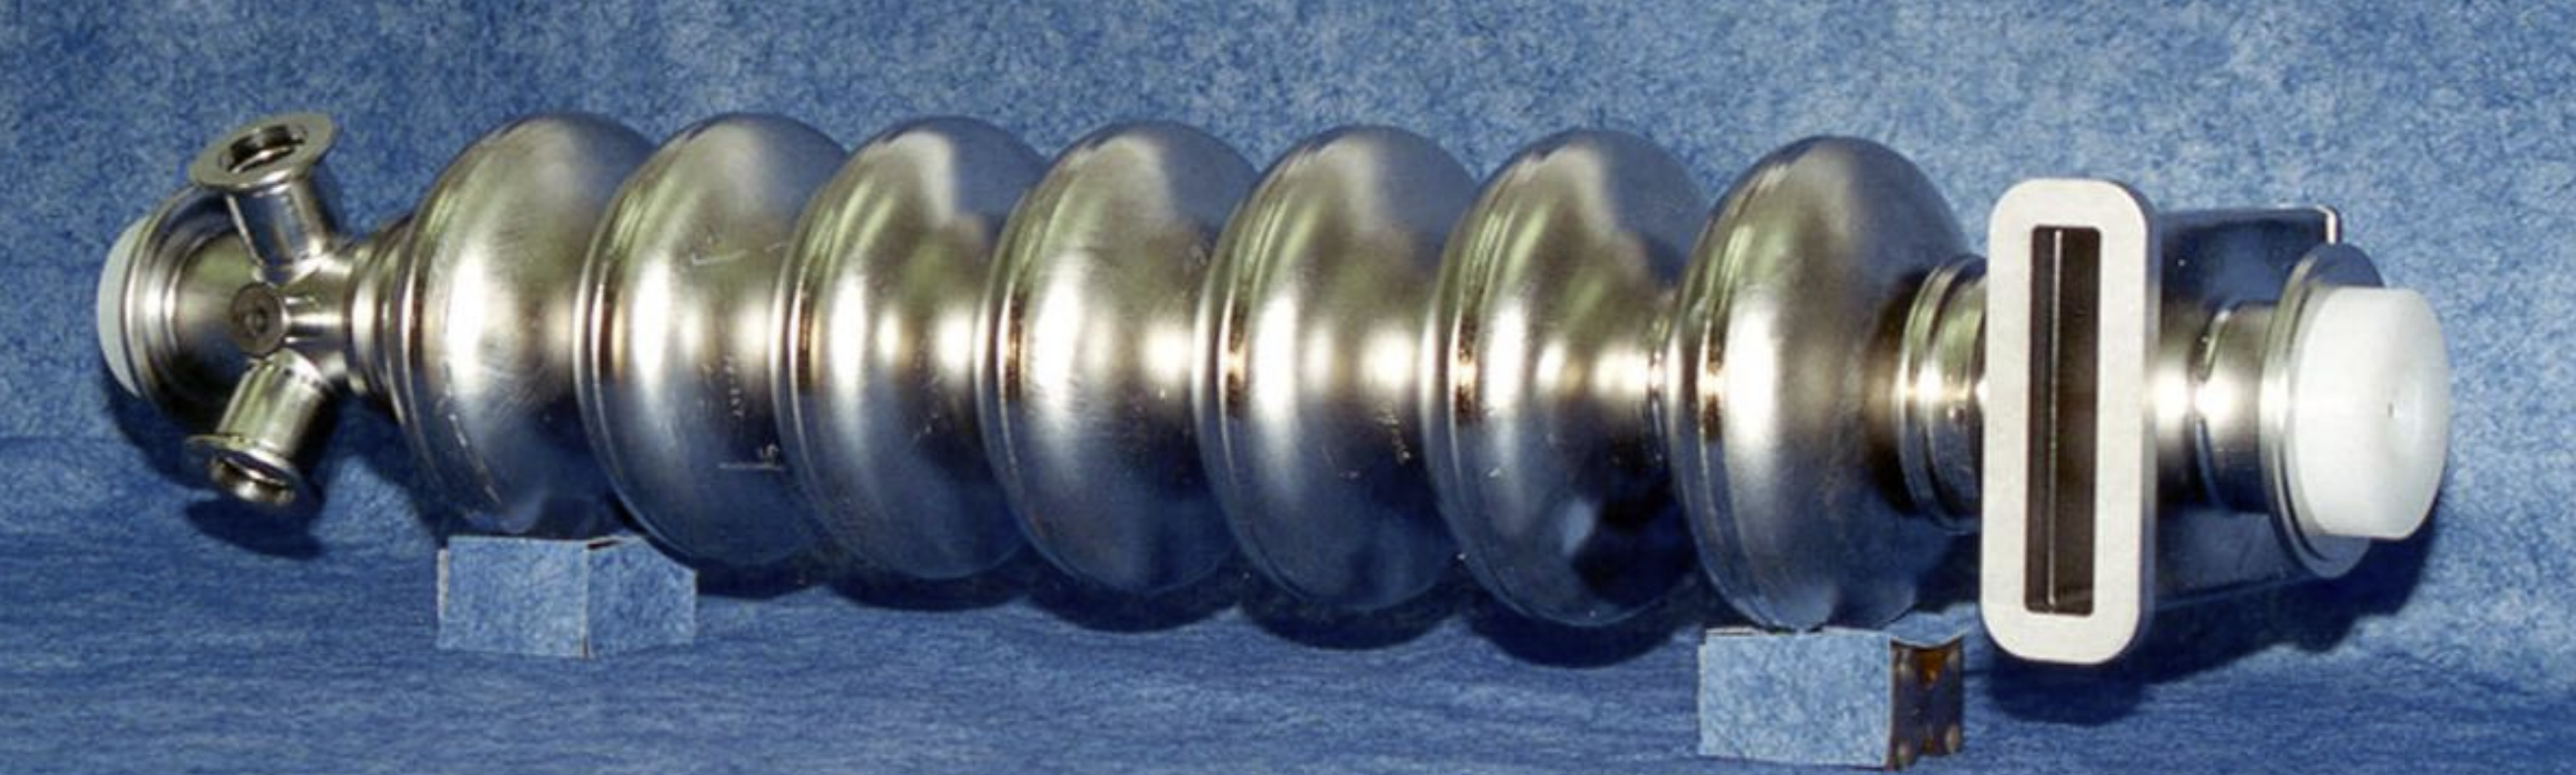
\includegraphics[width=0.4\textwidth]{Chapters/Ch2-Experiment/accel_and_beamline/pics/CEBAF/klystron.png}}
            \subfloat[]{\label{fig:magnets}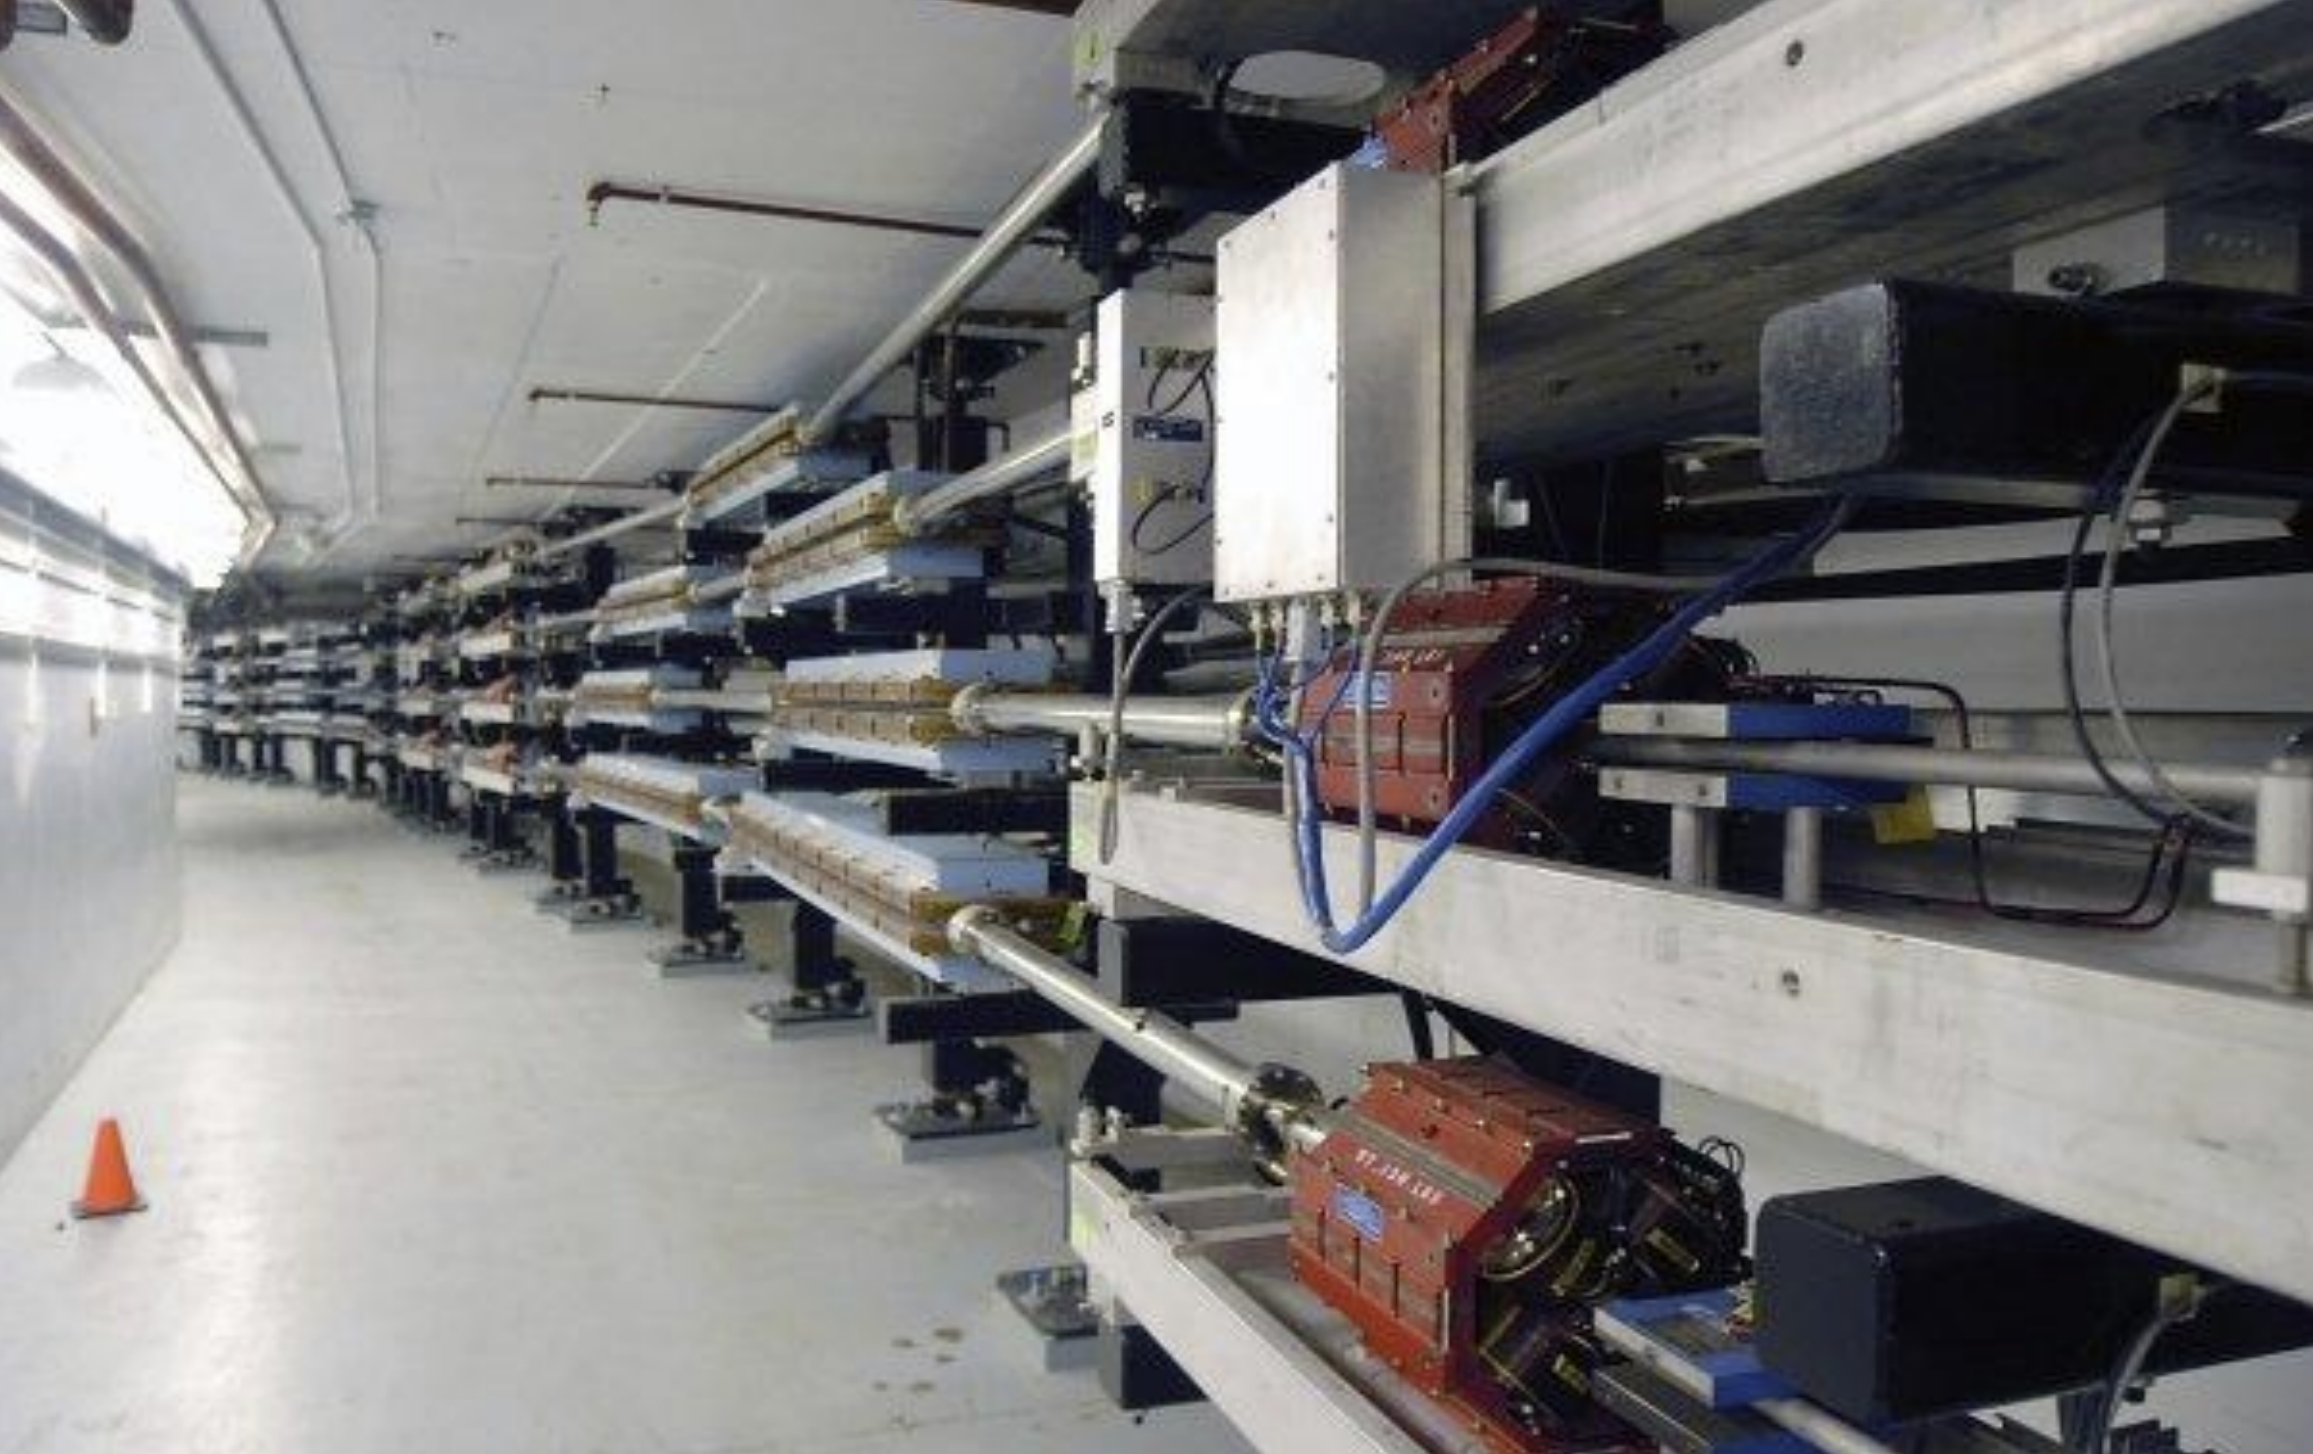
\includegraphics[width=0.4\textwidth]{Chapters/Ch2-Experiment/accel_and_beamline/pics/CEBAF/magnets2.png}}
        \end{minipage}
        \caption{(a) CEBAF guns, (b) Beam chopper, (c) Beam structure, (d) Superconducting resonator, (e) Dipole magnets.}
        \label{fig:JLab}
    \end{figure}
    

\subsection{Hall B Beamline}

    Moller polarimeters
    raster and target
    faraday cup / beamdump

    
    Finally, excess beam is safely managed using beam dumps. 
    
    \begin{figure}[ht]
        \centering
        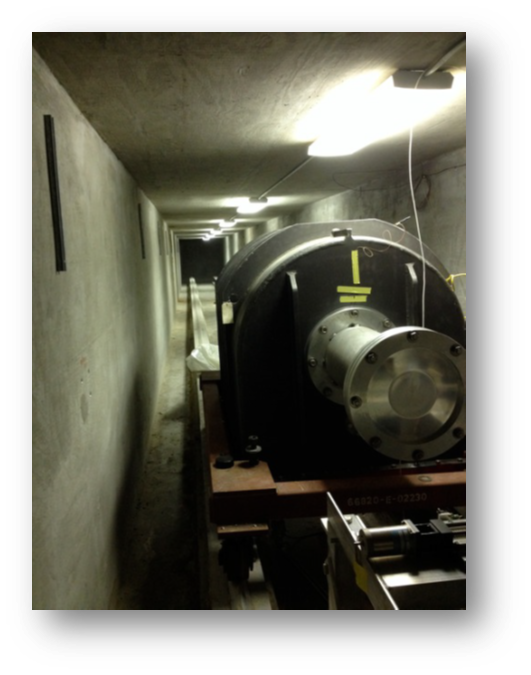
\includegraphics[width=0.8\textwidth]{Chapters/Ch2-Experiment/accel_and_beamline/pics/hallB/beamdump1.png}
        \caption{The first stage of the beam dump system at JLab.}
        \label{fig:beam_dump1}
    \end{figure}
    
    \begin{figure}[ht]
        \centering
        \includegraphics[width=0.8\textwidth]{Chapters/Ch2-Experiment/accel_and_beamline/pics/hallB/hall-b-poll-2.jpg}
        \caption{Moller polarimeters}
        \label{fig:beam_dump1}
    \end{figure}

    
    \begin{figure}[ht]
        \centering
        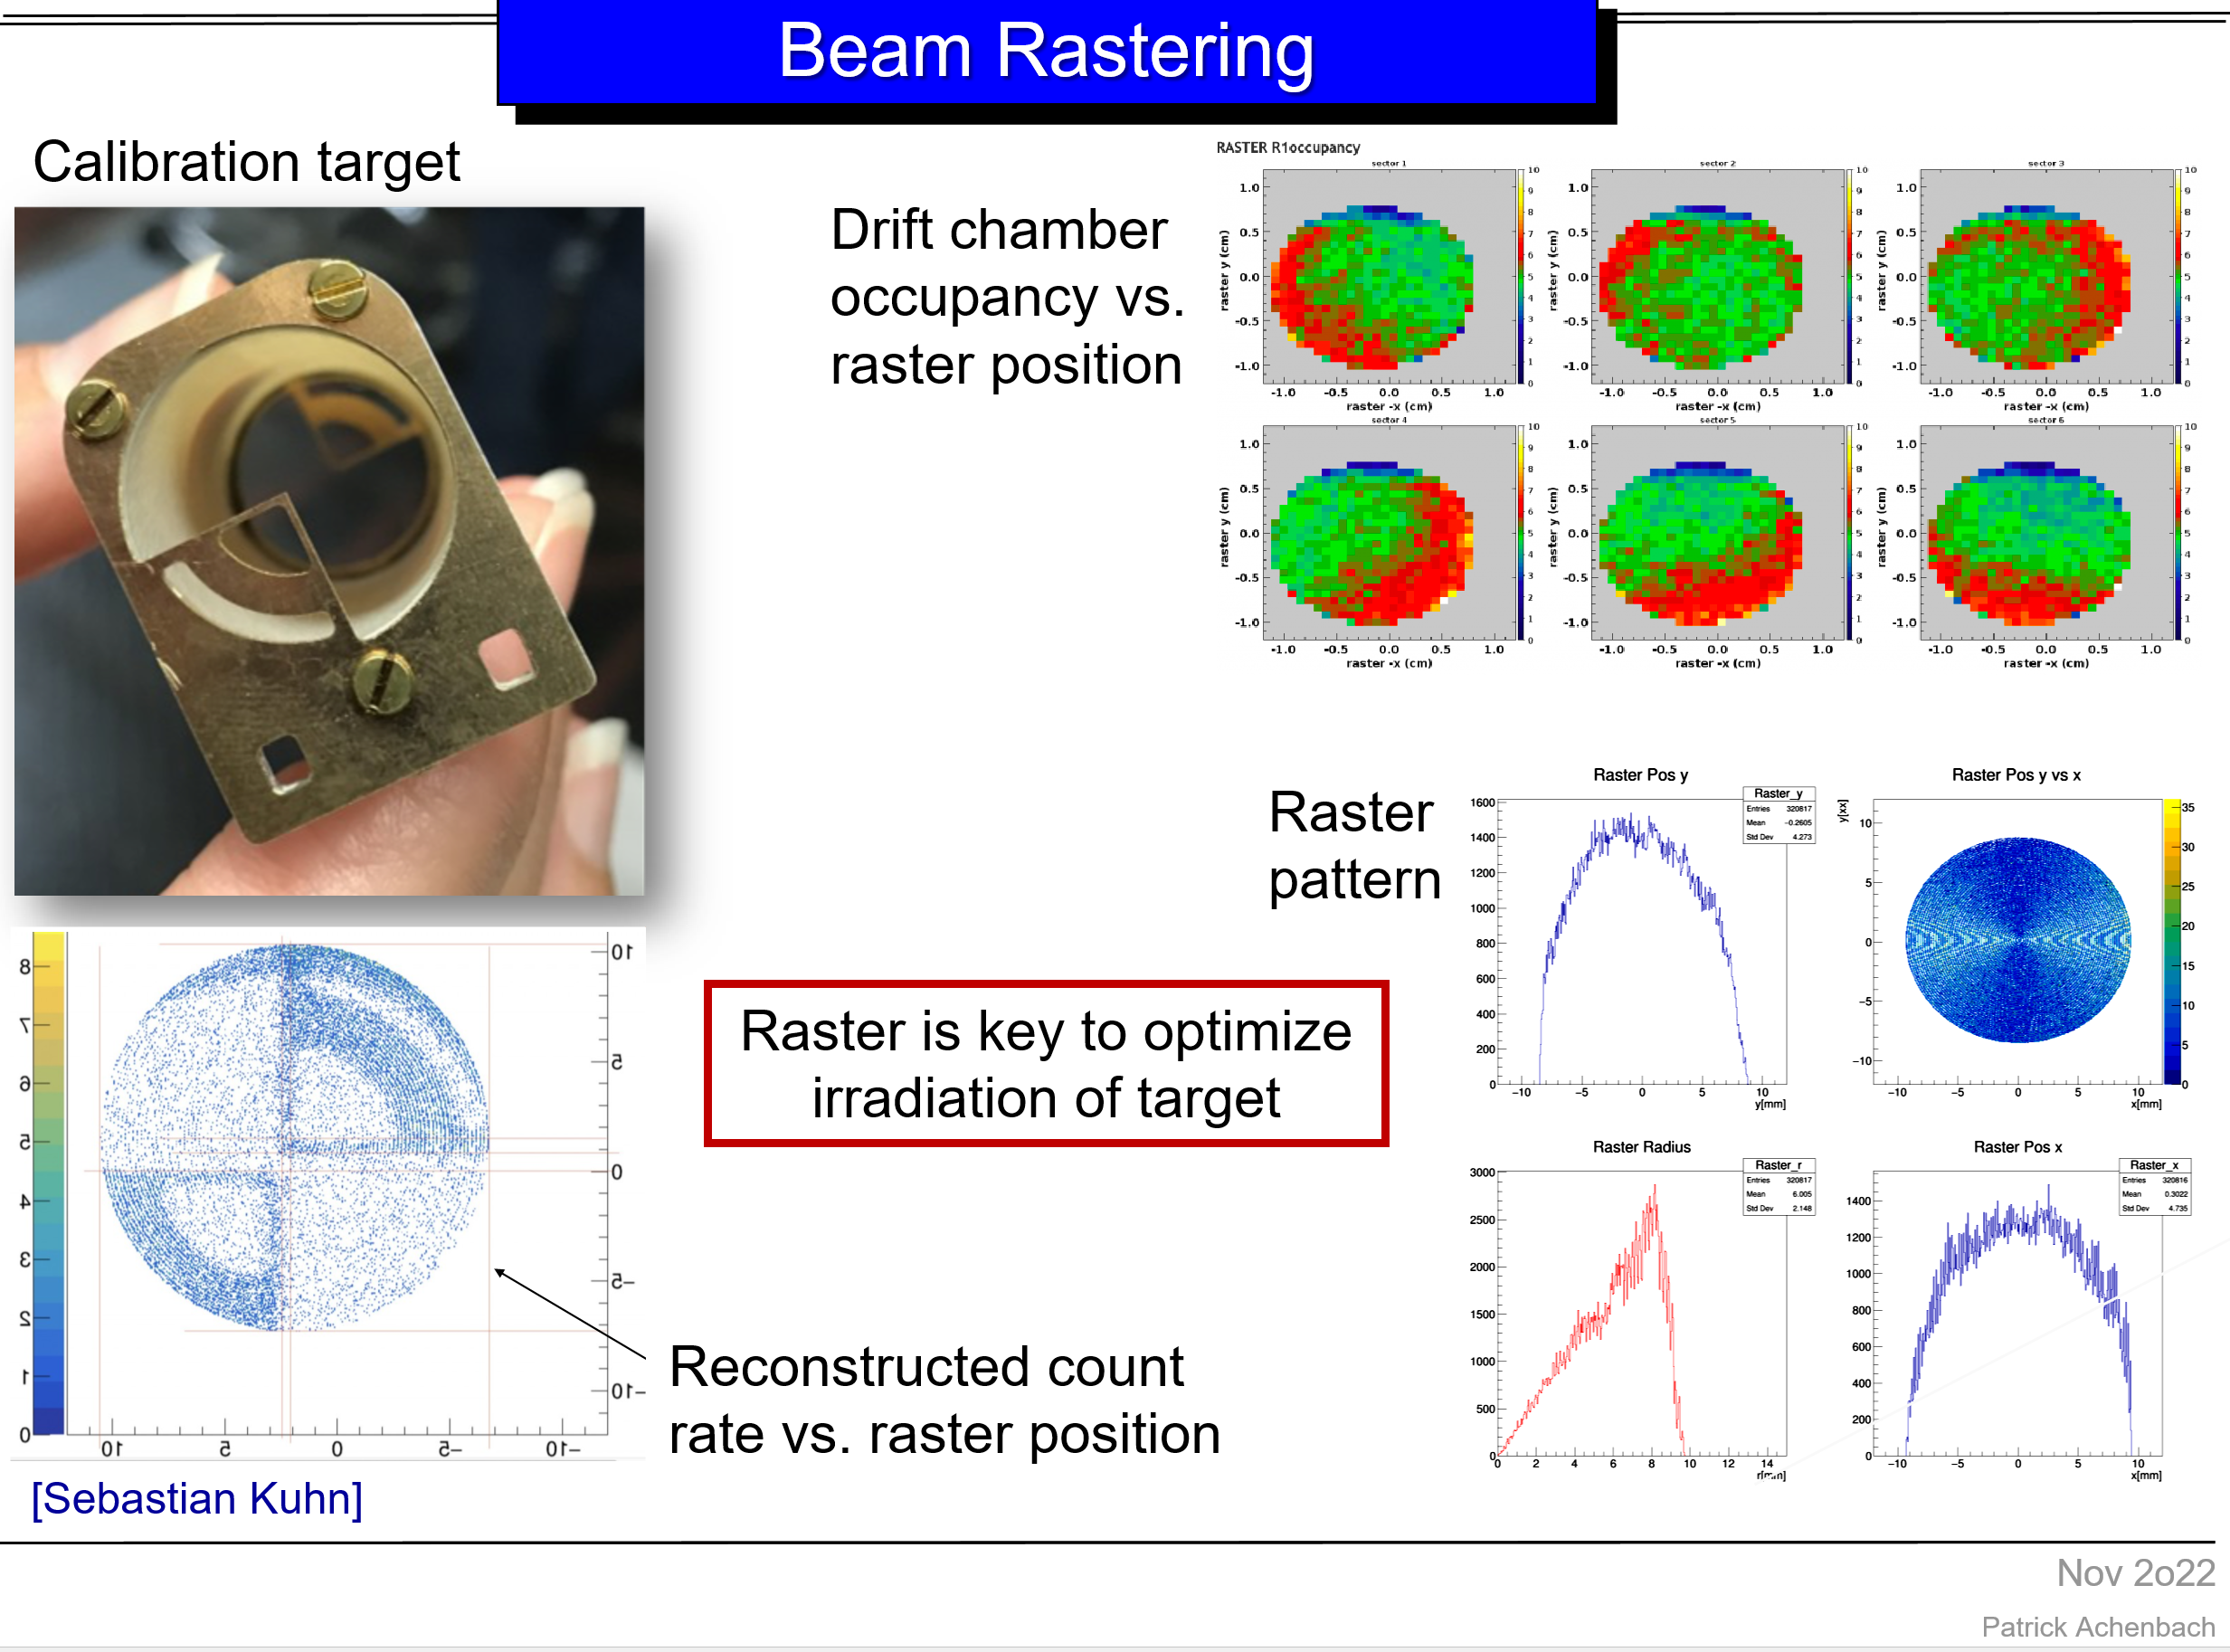
\includegraphics[width=0.8\textwidth]{Chapters/Ch2-Experiment/accel_and_beamline/pics/hallB/beam_rastering.png}
        \caption{The second stage of the beam dump system at JLab.}
        \label{fig:rastering}
    \end{figure}
    
    
    
        in beam dump area, link to own fraday cup paper \cite{Johnston2019RealizationElectrons}
        
    
    For entry into CLAS12, the beamline specs are as follows:\\
                        Beam current: up to 50 nA\\
                        Beam energy spread: $10^-4$\\
                        Beam size: Less than 0.4 mm\\
                        Beam stability: Less than 0.1 mm\\
                        Beam halo: $10^-4$\\
                        Beam polarization: up to 85\%\\
                        
    
    
    
    
    
     As stated, for RGA, the fact that the beam is polarized is not useful, but it is true and is measured by Moller Polarimeters. 
            
                Polarimietry: 
                        Good for beam energies between 100 MeV and 50 GeV. Polarized beam electrons are scat-
                tered from other polarized electrons in a target, usually magnetized foils. Only a small
                fraction of all the target electrons are polarized, so this method has a small analyzing
                power. Analyzing power is exactly calculable in QED. At high beam energies, analyzing
                power and scattering probability both become independently of beam energy. Maximum
                analyzing power is about 80%, maximum is at 90 degrees scattering angle in C.o.M. Trans-
                versely polarized target can be used to measure transverse beam polarization, but analyzing
                power is only about 10%. 90 degrees C.o.M. translates to a small lab angle with each elec-
                tron at half beam energy, so magnets are used to bend these electrons out to detectors.
                These detectors can be, for example lead glass total absorption cherenkov counters.Since
                the two electrons are corellated, can use things like time coincidence to reduce background,
                although for low duty factor accelerators only one electron is required as statistics would
                otherwise be too low.A main background to this process is Mott scattering with the electron
                radiating off energy after scattering, appearing as a Moller electron
                
                The scattering target is either iron or vanadium permendur (iron-cobalt alloy). Only 2 of
                26 electrons in iron have their spins oriented, leading to a total analyzing power of only 6 percent
                and transverse analyzing power of only 1%. Uncertainties in how magnetized the targets
                actually are corresponds to an uncertainty in analyzing power. There are ’easy’ and ’hard’
                magnetization schemes - easy does a soft magnetization, while hard uses a several tesla mag-
                net to saturate the target. In principle, uncertainties on magnetization in the hard scheme
                can be removed by using the Kerr magneto-optic effect, but this has not ever been imple-
                mented. An important correction is due to the Levchuk effect, where due to momentum
                differences between electrons in different shells, electrons scattered off of polarized electrons
                are more likely to be detected than off of unpolarized electrons. Specifically, inner electrons
                are unpolarized and have a large average momenta, so when struck they can fall outside the
                113 TOC
                acceptance of the Moller detectors, while the outer electrons, which are polarized, have a
                small average momentum, and behave as expected. This is up to a 15% effect on polarization
                measurements, and is currently a work in progress.
    
    
                
    
                 Rasterization of some kind
                    \\
                    \indent The hydrogen target in RGA is cooled to 20 K using a He4 evaporation fridge. Can by polarized by dynamic nuclear polarization, driven by a 140 GHz microwave source, can reach 90\% polarization for protons, 40\% for deuterons (both longitudinally polarized). The polarization can be measured by a Q-meter based NMR. 2.5 cm diameter target, extended 5 cm long. \\
                    \indent RGA does not use a polarized target. The beam is polarized, but the target is not, so polarization is not helpful for extracting the 5-fold differential cross section (but it would be if the target was also polarized, and is useful for BSA measurements).
                
       
                Luminosity in CLAS12 is measured from the Faraday Cup and using reference reactions such as elastic scattering. We don't use the Faraday Cup event by event, but we do use it run by run. For beam current measurements, beam position monitors upstream are used - but this is for monitoring on-line, not for analysis.
                           Can manage 175 Watts - 17 nA at 10 GeV. Is used to calibrate beam current, needs a blocker in at higher currents

\cleardoublepage
                                         

\section{CLAS Detectors and Run Conditions}\label{sec:clas12exp}
    \subsection{CLAS Detector System}
        
            \subsection{Forward Detector}
        Overview:
        \subsubsection{HTCC}
            Used basically as an electron trigger. Composed of 60 lightweight ellipsoidal mirrors, that focus Cherenkov light onto eigh 5-inch phototubes (48 channels on entire HTCC). Working gas is CO2 at STP (n=1.0005, $\theta_{max}$ = 1.7 degrees, covers 5 to 35 degrees, 2$\pi$ in azimuth. Active area 2.4 meters in diameter. Electron signal threshold is 15 MeV, charged pion threshold is 5 GeV. 99.9\% electron detection efficiency vs. pions. 15 feet in diameter, 6 feet long. Mirror thickness is 0.1 g/$cm^2$. Kaons have no signal, as they would need 16 GeV to generate a signal. Uses Winston cones to increase collection efficiency. 20 photoelectrons per electron in HTCC, 25\% quantum efficency. The PMTs have 14 dynodes, gain of about $10^7$. HTCC material budget 0.135 g/$cm^2$
            
            									
			 \begin{figure}[H]
    			\centering
    			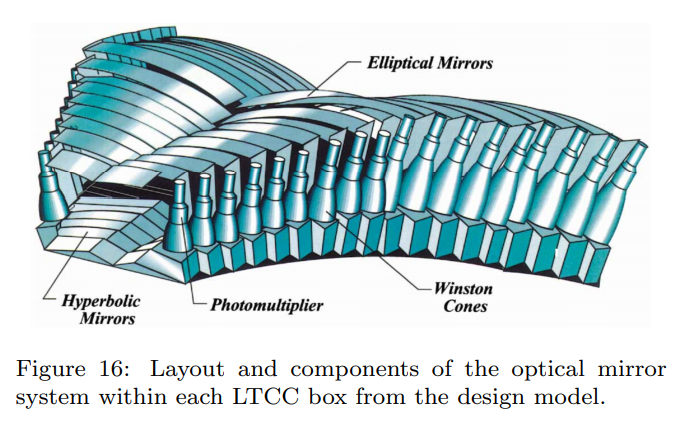
\includegraphics[width=12cm]{Chapters/Ch2-Experiment/clas-12-system/pics/fd/htcc-mirrors.PNG}
    			%%%\caption{SVT Strip}
			\end{figure}
			
						
									
			 \begin{figure}[H]
    			\centering
    			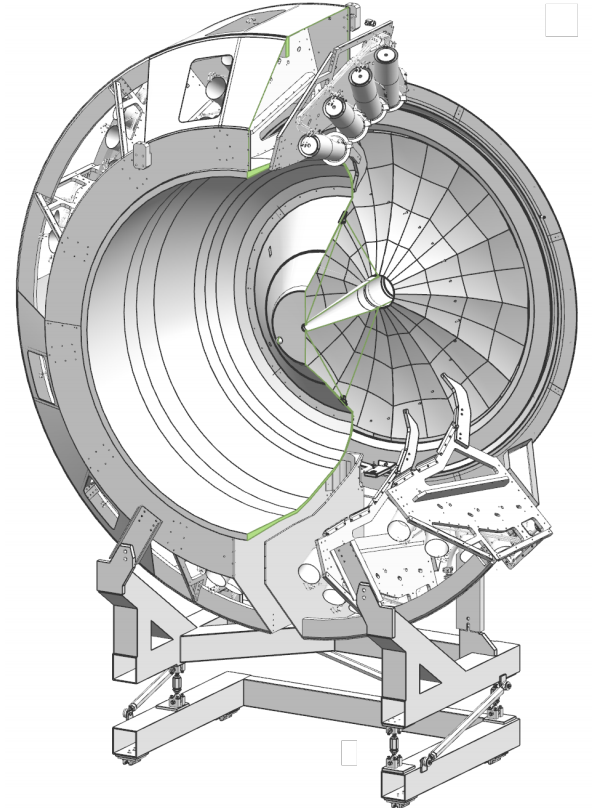
\includegraphics[width=12cm]{Chapters/Ch2-Experiment/clas-12-system/pics/fd/htcc.PNG}
    			%%%\caption{SVT Strip}
			\end{figure}
			
			

        
        \subsubsection{Torus}
        Outbending allows for lower Q2 measurements, inbending allows for slighly higher Q2 measurements. 

            6 coil torus, 4k amps, 3.5 Tesla torodial field, supercritical LHe cooled. 14.2 Megajoules stored energy. 2 Henries of inductance. Field strongest at small angles, weakest at large angles. 
              Inbending vs out bending:
        I have been wondering about this as well. All I know is that inbending and outbending have different acceptances.
        So, I guess some channels prefers inbending while the others do outbending? I’m not sure though. FX claims outbending results have better quality for these days. 
            									
			 \begin{figure}[H]
    			\centering
    			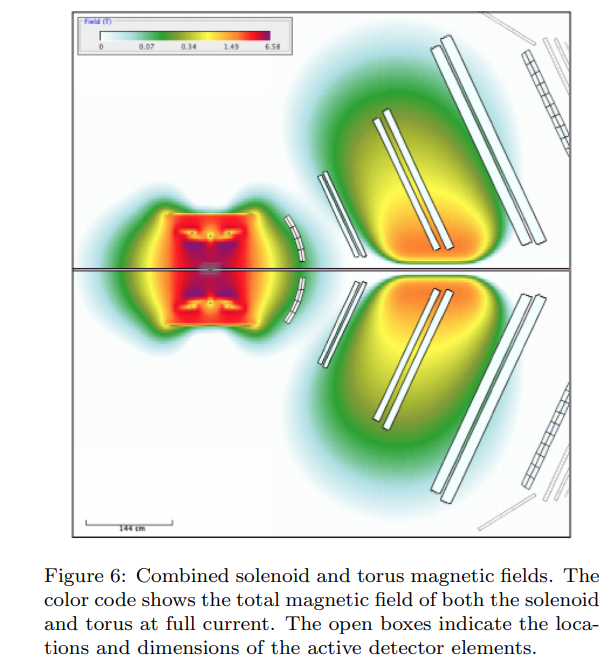
\includegraphics[width=12cm]{Chapters/Ch2-Experiment/clas-12-system/pics/fd/torus.PNG}
    			%%%\caption{SVT Strip}
			\end{figure}
                        

        
        \subsubsection{Drift Chambers}
            There are 3 layers of drift chambers, each with 6 sections. Each chamber has 2 superlayers of 6 layers by 112 wires, for a total of 24,192 wires. (Structure is 112 wires * 6 layers * 2 superlayers * 18 DC sections = 24,192 wires). Physical wire sectioning looks like:\\
            (IIIIII)-(IIIIII)---(IIIIII)-(IIIIII)---(IIIIII)-(IIIIII) x 6 sectors\\
            Where each "I" is a layer of 112 wires.\\
            Spatial resolution is 300 $\mu$ m, angular coverage 5-40 degrees. Momentum resolution $\Delta$p/p < 1\%, angular resolution is 1 mrad in theta, 1mrad/$\sin{\theta}$ for phi. The Drift Chambers are located 2, 3, and 4 meters from the gas mixture is 90/10 Argon/CO2. Time resolution = ?\\
            DC specifics: 30 micron diameter tungsten sense wires, 80 micron Cu-Be field wires, 140 micron Cu-Be guard wires. 20 g tension on sense, 62 g tension of field, 180 g on guard. Max sag calculated to be on order of 10 microns.
            
            									
			 \begin{figure}[H]
    			\centering
    			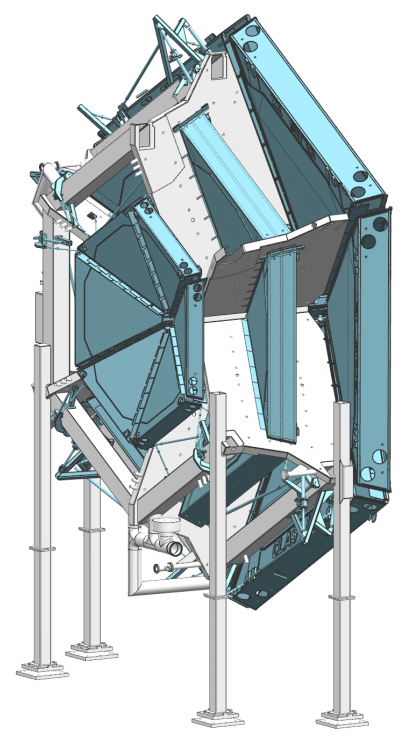
\includegraphics[width=12cm]{Chapters/Ch2-Experiment/clas-12-system/pics/fd/drift-chambers.PNG}
    			%%%\caption{SVT Strip}
			\end{figure}    

            
        \subsubsection{LTCC}
            6 sectors, perfluorobutane ($C_4F_10$) $\longrightarrow$ n = 1.0013 $\longrightarrow$ $\theta_{max}$ = 3 degrees. Electron threshold 9 MeV, pion threshold 2.7 GeV, Kaon threshold 9.4 GeV. Allows for good pion/kaon discrimination from 3.5 Gev to 9 GeV. \\
            Each section has 108 mirrors, 36 winston cones, and 36 PMTs. Mirror is aluminium with $MgF_2$ coating. Kevlar support structure. Perflourobutane is 100\% transparent above 220 nm light. 
            
            
						
									
			 \begin{figure}[H]
    			\centering
    			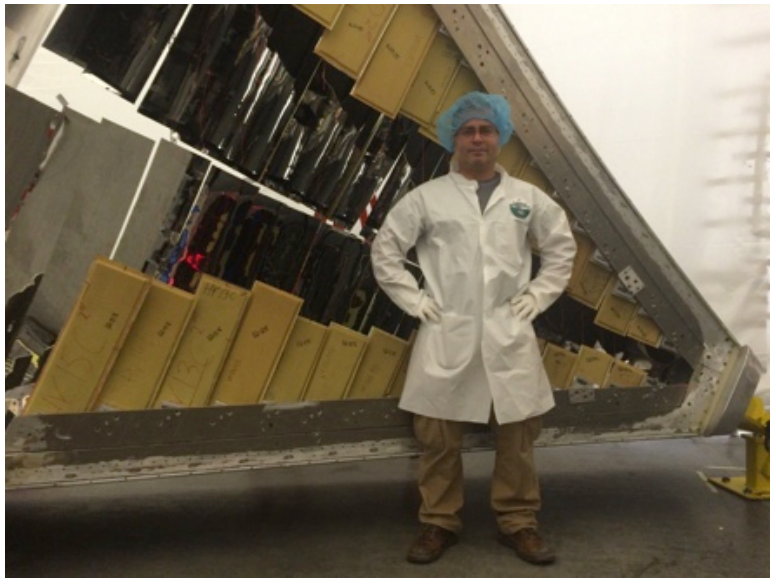
\includegraphics[width=12cm]{Chapters/Ch2-Experiment/clas-12-system/pics/fd/ltcc.PNG}
    			\caption{Low Threshold Chrenkov Counter}
			\end{figure}
			
			

			
        \subsubsection{RICH}
            Provides PID in the range of 3-8 GeV, replacing one sector of LTCC (right middle sector). Pion/Kaon rejection factor > 500, Kaon/Proton rejection factor > 100. Covers 5 to 25 degrees in theta, uses aerogel (n=1.05 $\longrightarrow$ $\theta_{max}$ = 18 degrees). Pion threshold 460 MeV, Kaon threshold 1.6 GeV. Read out by 64 channel photomultipliers. $\beta_{min}$=0.95, $\gamma_{min}$ = 3.3
            
            What is angular resolution?
            
            Reminder of relevant equation:
            \begin{equation}
                \cos{\theta} = \frac{1}{\beta n} \longrightarrow \theta = \arccos{\frac{1}{\beta n}}
            \end{equation}
            
            \begin{equation}
                \gamma = \frac{1}{\sqrt{1-\beta^2}} \longrightarrow \beta = 1-\frac{1}{1-\gamma^2} 
            \end{equation}
            
            \begin{table}[H]
                \centering
                    \begin{tabular}{llll}
                         & momentum & $\sim \gamma$ & $\theta$  \\
                    pion & 3        & 21            & 17.4                      \\
                    kaon & 3        & 6             & 12                        \\
                         &          &               &                         \\
                    pion & 5      & 36            & 17.6                      \\
                    kaon & 5       & 10.1             & 15.9                        \\
                         &          &               &                          \\
                    pion & 8      & 57.1            & 17.7                      \\
                    kaon & 8       & 16             & 17.1                        \\
                    
                    \end{tabular}
            \end{table}
            
        
            
            
            
            \begin{table}[H]
                \centering
                    \begin{tabular}{lll}
                        Detector    &   Scintillator                         &   PMT   \\
                        FTOF - 1a   &     \textcolor{blue}{BC-408}           &   \textcolor{red}{Phillips XP2262, EMI 9954A}\\
                        FTOF - 1b   &     \textcolor{red}{BC-404}           &   \textcolor{blue}{Hama. R9779} \\
                        FTOF - 2    &     \textcolor{blue}{BC-408}           &   \textcolor{magenta}{EMI 4312KB} \\
                        PCAL        &     FNAL                               &   \textcolor{red}{Hama. R6095}\\
                        ECAL        &     \textcolor{cyan}{BC-412}           &   \textcolor{red}{Philips XP2262, EMI 9954}\\
                        CND         &     \textcolor{red}{EJ-200}            &   \textcolor{cyan}{Hama. R10533} \\
                        CTOF        &     \textcolor{blue}{BC-408}           &   \textcolor{green}{Hama. R2083} \\
                        HTCC        &         N/A                            &   ET 9823QKB \\
                        LTCC        &           N/A                          &   200 Photonis XP 4500B\\
                        LTCC        &              N/A                       &   16 Photonis XP 4508 (Quartz Window)\\
                    \end{tabular}
            \end{table}
            
            *ET stands for Electron Tube, a company. Could not find a spec sheet for this PMT type. 
            ** Could not find spec sheets for either HTCC, or LTCC PMTs. 
       
               
            \begin{table}[H]
                \centering
                    \begin{tabular}{lllllll}
                        Scintillator                    & Detectors             &   Principal Use/Features      &   L.O. & WME & R/D Time & L.A. Length \\
                         \textcolor{red}{BC-404}       &  FTOF-1b              &   Fast Counting                   &           68    &   408    & 0.7/1.8           &   140   \\
                         \textcolor{blue}{BC-408}       &  FTOF-1b,2,CTOF       &   TOF - Large Area                &           64    &   425   &   0.9/2.1         &   210  \\
                        \textcolor{cyan}{BC-412}        &  ECAL                 &   Large Area                      &           60   &   434 &   1.0/3/3         &   210\\
                        \textcolor{red}{EJ-200}        &  CND                  &   Long attenuation, fast   &           64     &   425       &   0.9/2.1         &   380   \\
                    \end{tabular}
            \end{table}   
            
            L.O - Light Output - \% Anthracene
            WME - Wavelength Maximum of Emitted Photons
            R/D Time - Rise / Decay time (ns)
            L.A. Length - light attenuation length (cm)
             
             All scintillators have a PVT (Polyvinyltoluene) base. 
             
             EJ-200:          200 -- 10K photons per 1 MeV. 
             
             Thermal effects: EJ-200 loses 5\% of its light output between 20 degrees C and 60 degrees C. No change between -60 to 20 degrees C. 
            
            \begin{table}[H]
                \centering
                %\begin{localsize}{10}
                \scalebox{0.9}{
                    \begin{tabular}{llllllll}
                        PMT                                         & Det.                      &       TS/A    &   WVE         &   PHTC    &   DNY     &       Anode  &    Time Resp.\\ 
                        \textcolor{red}{Hama. R6095}               &  PCAL                     &       28/25   &   300/420/650 & BA/BSG & B\&L/11/2.1  &   1500/0.1    & 4/30/3    \\
                        \textcolor{blue}{Hama. R9779}               &  FTOF-1b                  &       51/46   &   300/420/650 & BA/BSG & LF/8/0.5     &   1750 /0.1   & 1.8/20/0.25 \\
                        \textcolor{cyan}{Hama. R10533}              &  CND                      &       51/46   &   300/420/650 & BA/BSG & LF/10/4.2    &   1000/0.1    &  2/24    \\   
                        \textcolor{green}{Hama. R2083}              &  CTOF                     &       51/46   &   300/420/650 & BA BSG & LF/8/2.5     &   3000/0.2    & 0.7/16/    \\
                        \textcolor{red}{Phillips XP2262}            &  FT1a ECAL            &    &&&&&\\
                        \textcolor{red}{EMI 9954A}                  &  FT1a ECAL            &    &&&&&\\
                        \textcolor{magenta}{EMI 4312KB}             &  FTOF-2                   &    &&&&&\\
                    \end{tabular}}
                %\end{localsize}
            \end{table} 
            
            No spec sheets could be found for the PMTs used in the TFOT1a, ECAL, or FTOF-2.
            Typical dark currents for all PMTs are 100 nA. 
        
            
            Tube size / photocathode area (diameter in mm)
            Wavelength short / peak / long (nm)
            Photocathode / window material (BA = Bialkali, BSG = Borosilicate Glass)
            Dynode structure / stages / gain  LF = Linear-focused, B\&L = Box and line / / Gain - Gain x 10$^6$
            Anode to Cathode Voltage / Anode Current  - Volts / mA
            Rise / transit time/time spread in ns
            
            
            
            \href{https://www.hamamatsu.com/eu/en/product/type/R10533/index.html}{R10533 PMT}
            \href{https://www.hamamatsu.com/eu/en/product/type/R2083/index.html}{R2083 PMT}
            \href{https://pdf1.alldatasheet.com/datasheet-pdf/view/212324/HAMAMATSU/R9779.html}{R9779 PMT}
            \href{https://www.sphere.bc.ca/test/phototubes2/ham/r6095.pdf}{R6095 PMT}
            
            
            
            
            
            
            
            
            
            \href{https://eljentechnology.com/products/plastic-scintillators/ej-200-ej-204-ej-208-ej-212}{CND Scintillator}
            
            
            \href{https://www.crystals.saint-gobain.com/sites/imdf.crystals.com/files/documents/bc400-404-408-412-416-data-sheet.pdf}{BC Scint Specs from Saint Gobain}
            
            
            \href{https://www.hamamatsu.com/eu/en/product/type/R10533/index.html}{CND PMT}
            
            
            \href{https://www.hamamatsu.com/us/en/product/type/R2083/index.html}{CTOF PMT Spec sheet}
            Bialkali photocathode, 8 dynodes, 2.5*10$^6$ typical gain
            Linear-focused dynode structure
            Window material Borosilicate glass
            peak wavelength 420 nm, range from 300 to 650 nm. Max anode to cathode voltage of 3500 V, made anode current of 0.2 mA. Dark current around 100 nA. 
            
            
        
        \subsubsection{FTOF}
            Used for PID, three layer system - 1a, 1b, and 2. Has a design resolution of 60 ps to 160 ps. Average scintillation rate 250 kHz. Pion/Kaon separation up to 2.8 GeV, Kaon Proton separation up to 4.8 GeV, pion proton separation up to 5.4 GeV. \\
            6 meters away from target.
            Time resolution of 80 ps less than 36 degrees, 150 ps greater than 36 degrees. PMTs are shileded from CLAS12 torus. 6 sectors, plastic scintillator, double sided PMT readout. 3 panesl - 1a - 23 counters, 1b - 62 counters, 2 - 5 counters. \\
            15cm wide x 5 cm deep x 33 cm up to 376 cm long.\\
            20-30 cm up to 15x5 130 ps\\
            350-400 cm 6x6 60 ps\\
            370 to 430 cm, 22x5cm, 150 ps\\
            
            									
			 \begin{figure}[H]
    			\centering
    			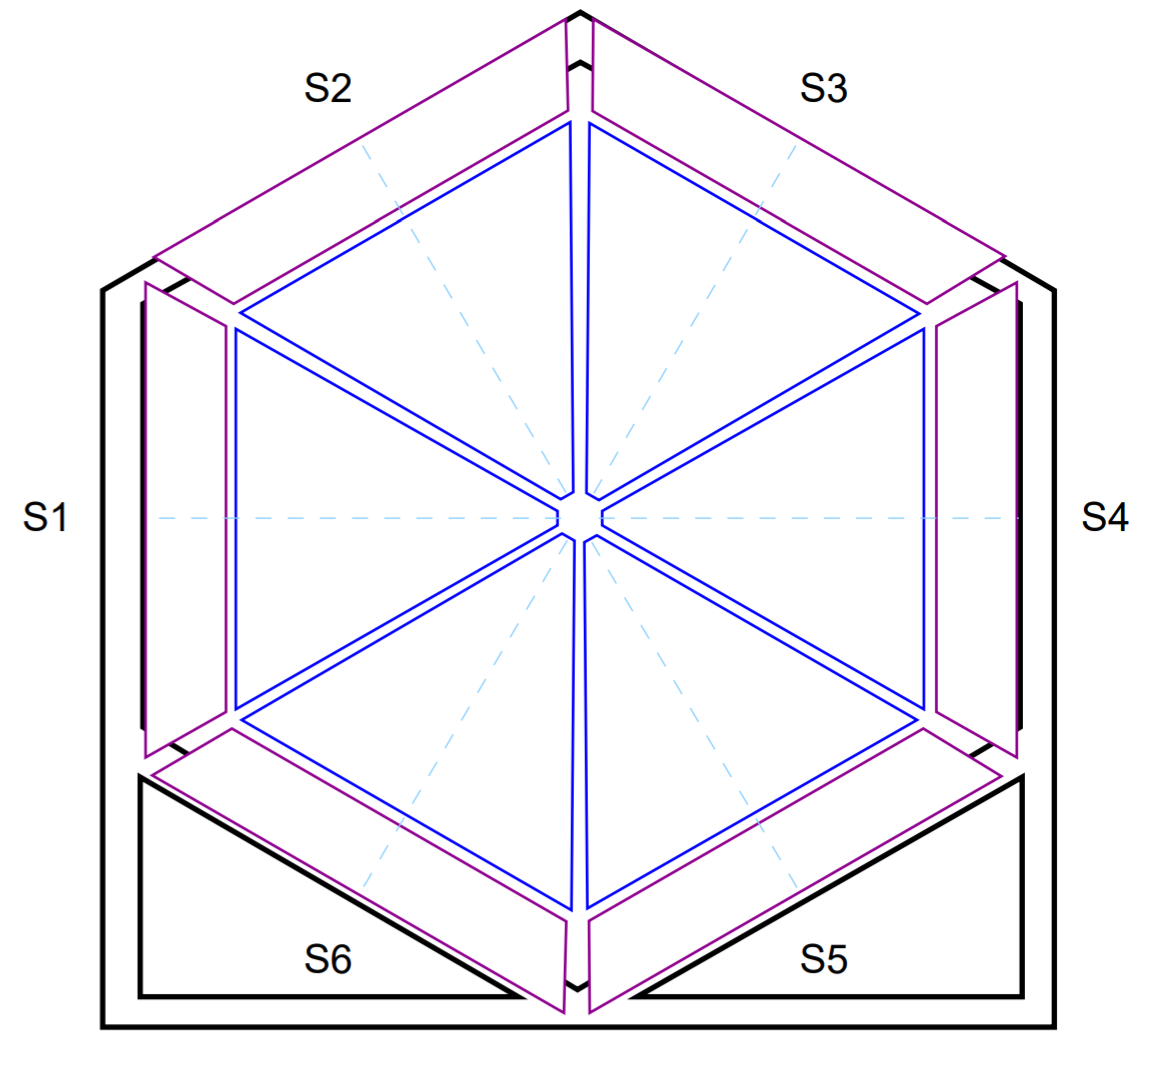
\includegraphics[width=12cm]{Chapters/Ch2-Experiment/clas-12-system/pics/fd/ftof-front.PNG}
    			%%%\caption{SVT Strip}
			\end{figure}

		
			 \begin{figure}[H]
    			\centering
    			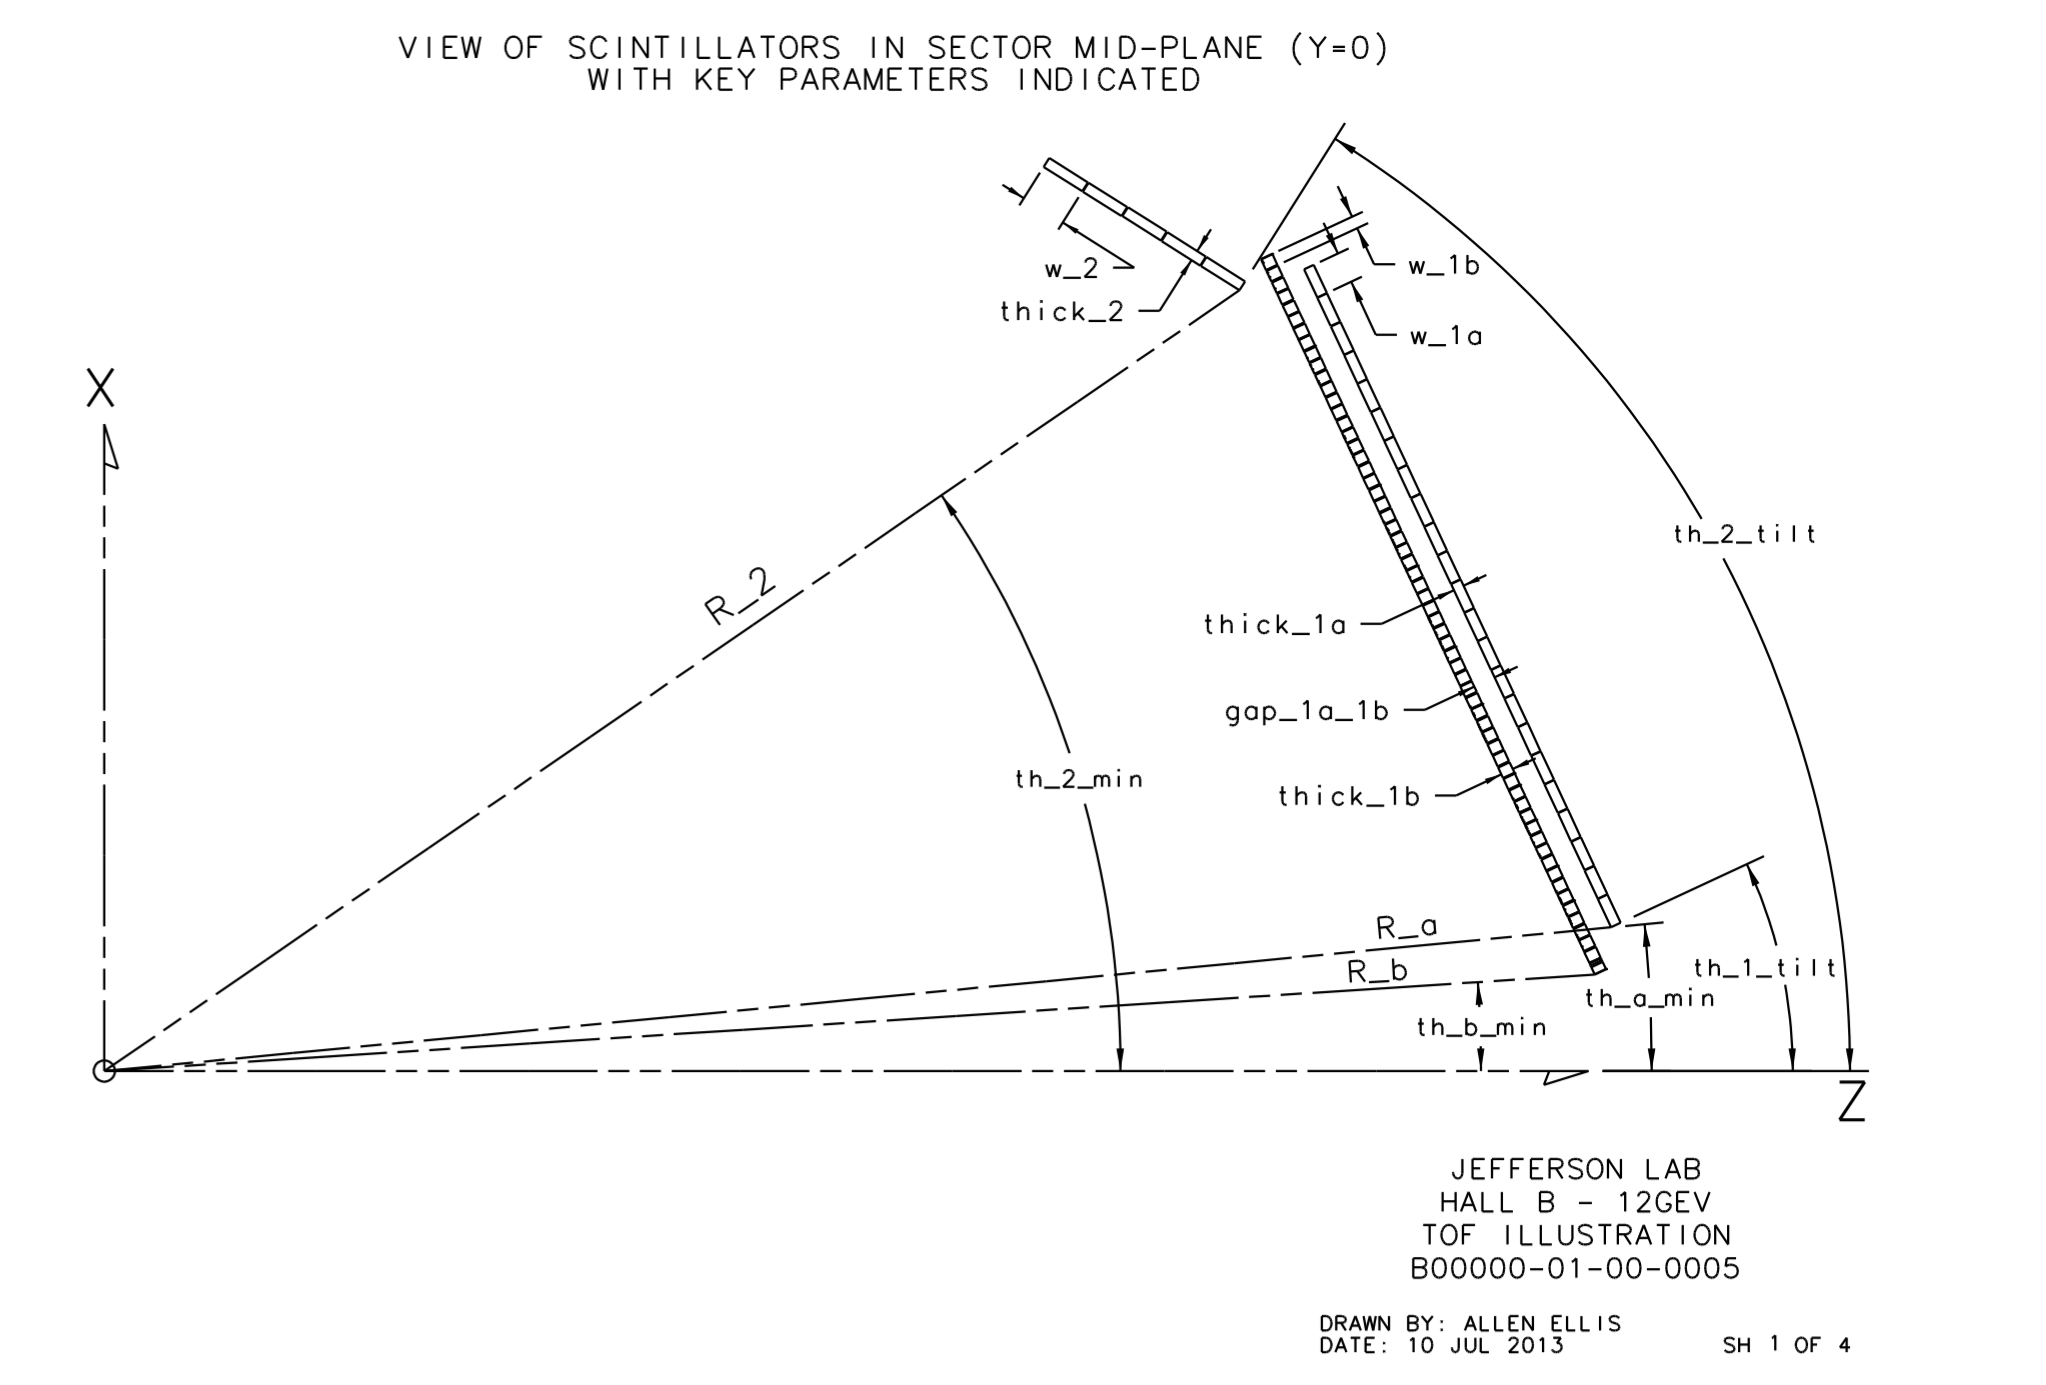
\includegraphics[width=12cm]{Chapters/Ch2-Experiment/clas-12-system/pics/fd/clas12-ftof-geom.PNG}
    			%%%\caption{SVT Strip}
			\end{figure}
			
			
            
            The timing resolution minimums are for being close to the beam axis where particles are moving faster, and farther out from the beamline (larger theta) particles are moving slower so a less resolved time difference is acceptable. 
            
            \paragraph{1a}
                Coverage is 50\% at 5 degrees to 85\% at 35 degrees\\
                Dimensions: L 32.3 cm to 376.1 cm, wxh = 15x5 cm\\
                Material BC-408\\
                PMTS: EMI 9954A, Phillips XP2262\\
                Time resolution 90 - 160 ps small bar to big bars\\
            \paragraph{1b}
                Coverage is 50\% at 5 degrees to 85\% at 35 degrees\\
                Dimensions: L 17.3 cm to 407.9 cm, wxh = 6x6 cm\\
                Material BC-404 (first half) and BC-408\\
                PMTS: Hamamatsu R9779\\
                Time resolution 60-110 ps small bar to big bars\\
            \paragraph{2}
                Coverage is 85\% at 35 degrees to 90\% at 45 degrees\\
                Dimensions: L 371.3 cm to 426.2 cm, wxh = 22x5 cm\\
                Material BC-408\\
                PMTS: EEMI 4312KB\\
                Time resolution 140 - 165 ps small bar to big bars\\
           
           
            For more FTOF specifcications, look \href{https://www.jlab.org/Hall-B/ftof/notes/ftof_geom.pdf}{here} 
                
            FTOF two panels:
Official answer from CLAS12 FTOF NIM paper:
"For tracks that pass through both arrays the combined time information (described in Ref. [10]) is used and results in a 20% improvement compared to using the hit information from panel-1b alone.”, https://www.sciencedirect.com/science/article/pii/S0168900220302102

I guess this is the right answer though:
1a is recycled one from CLAS while 1b is new one.
            
            
        \subsubsection{PCal and ECal}
            ECal from CLAs could only contain showers with E < 5 GeV. Above 5.5 GeV, couldn't resolve neutral pion gamma gamma angle, so needed PCAL. PCAL is 7 meters from target, ECAL is 7.5 M from target. EC segmentation 10 cm, PCAL finer segmentation. PCal 5.5 radiation lengths. 20.5 radiation lengths total. Both are sampling calorimeters, with PB and scintillator layers. The CLAS ECAL was resused and a new PCAL was installed in front of it. Primarily used for identification of electrons, photons, gamma gamma decays from pions, and neutrons. They are sampling calorimeters with six moduels. Each module has a triangular shape with 54 (15/15/24 - PCAL/ECALinner/ECALouter) layers of 1 cm htick scintillators segmented into 4.5/10 cm (PCAL/ECAL) wide strips and sandwiched between 2.2 mm thick lead sheets. The total thickness is about 20.5 radiation lengths. \\
            \indent Scintillator layers are grouped into three readout views with 5/5/8 PCAL/ECinner/ECouter, layers per view providing several cm resolution of energy clusters. Light from each scintillator readout group is routed to PMTs via flexible optical fibers.\\
            Overall perfomance:\\
            Energy resolution of 10\%, position resolution of 2 cm, time resolution of 500 ps. \\
            Are these the real statistics? Because they seem like BS.
            
            
            
            \begin{figure}[H]
    			\centering
    			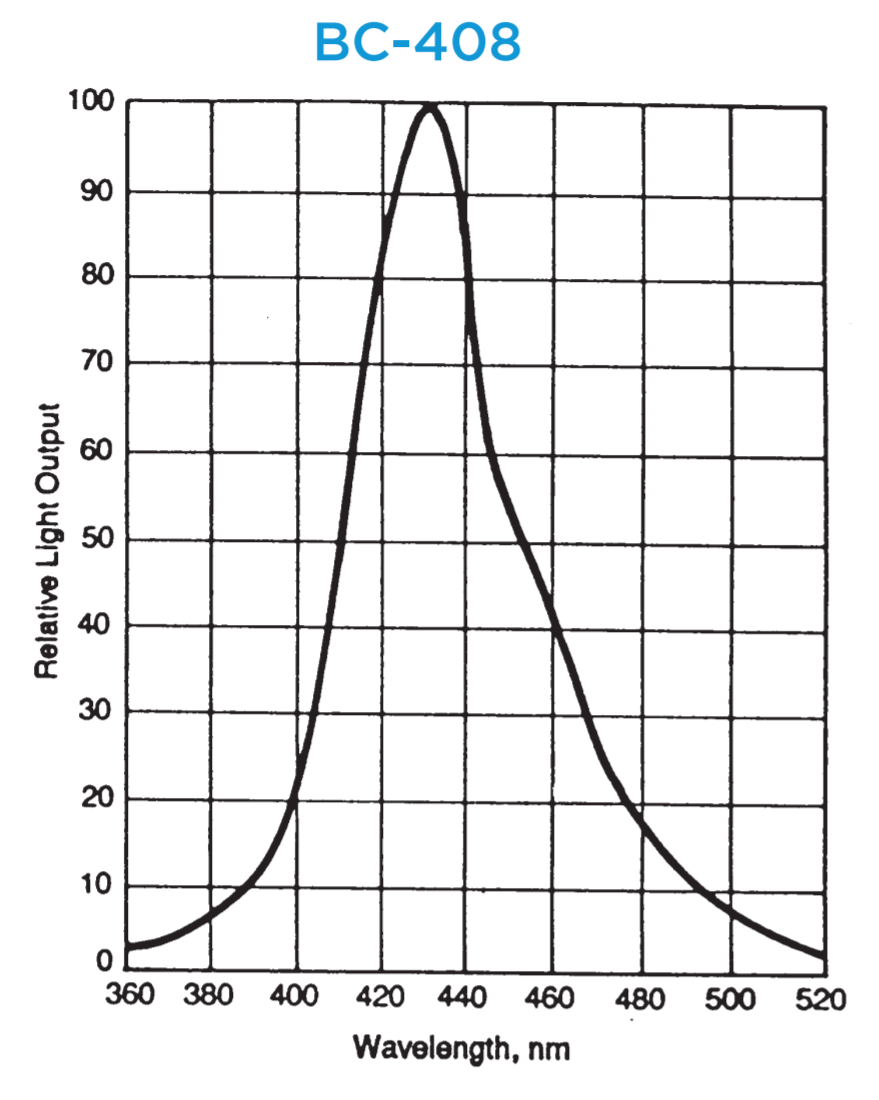
\includegraphics[width=12cm]{Chapters/Ch2-Experiment/clas-12-system/pics/fd/sample-BC-408-emission-spectra.PNG}
    			%\caption{BC 408 Emission Spectra}
			\end{figure}
			
            						
									
			 \begin{figure}[H]
    			\centering
    			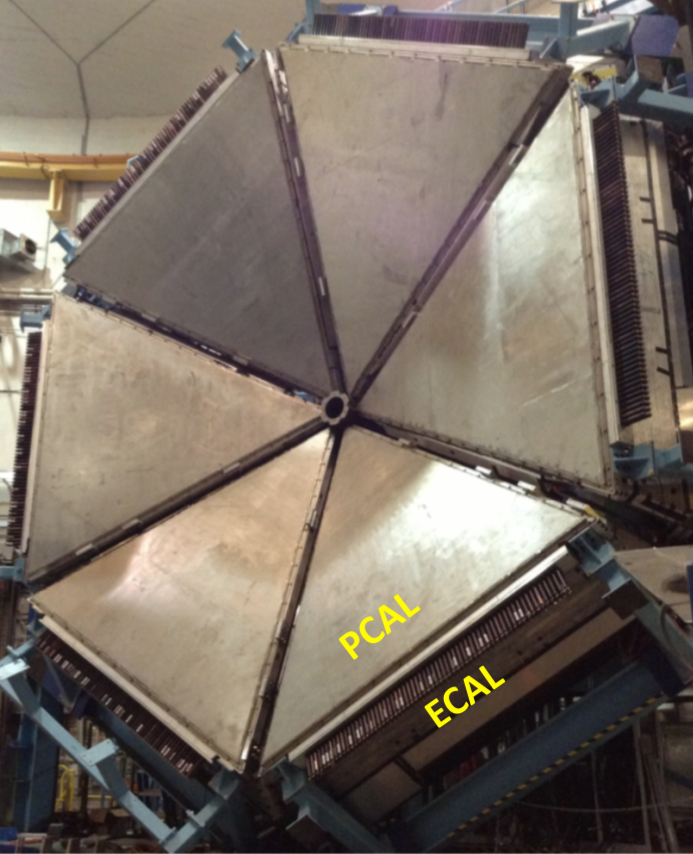
\includegraphics[width=12cm]{Chapters/Ch2-Experiment/clas-12-system/pics/fd/clas12-pcal-ecal.PNG}
    			%%%\caption{SVT Strip}
			\end{figure}
			
			
        \subsubsection{PCAL}
                \indent 50\% coverage at 5 degrees, 85\% coverage at 35 degrees. 15 scintillators, 14 lead layers, per module. 1200 scintillator strips, 1x4.5 cm$^2$ up to 432 cm long, with two holes along the strip, and 0.25 mm TiO2 coating (reflective coating)\\
                Lead sheets are 2.2 mm thick. Readout by fibers into 1 inch PMTs, Hamamatsu R6095. Light yield is 11-12 photo-electrons per MeV. 
                
                PCAL scinitllator was manufactured at the FNAL-NICADD Extrusion Line Facility. Polystyrene base was Dow STYRON 663 W, primary dopant is 2,5 -diphenyloxazole (PPO, 1\% by weight) - this is the organic scintillator, peaks at 385 nm:
                
                
            \begin{figure}[H]
    			\centering
    			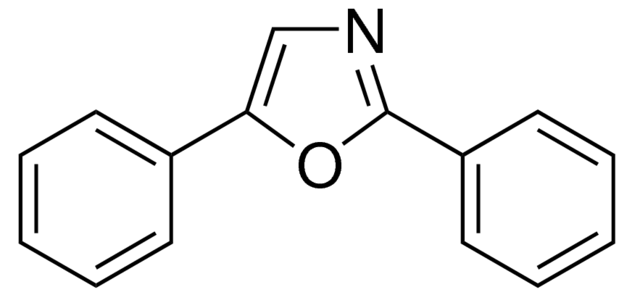
\includegraphics[width=12cm]{Chapters/Ch2-Experiment/clas-12-system/pics/fd/2-5-diphenyloxazole.png}
    			%\caption{2,5-diphenyloxazole}
			\end{figure}
                
                The Secondary dopant is 1,4 bis (5-phenyloxazol- 2-yl) benzene (POPOP, 0.03\% by weight) - also scintillator, peaks at 410 nm. 
                
                                
            \begin{figure}[H]
    			\centering
    			
\includegraphics[width=12cm]{Chapters/Ch2-Experiment/clas-12-system/pics/fd/popop.png}
    			%\caption{1,4 bis (5-phenyloxazol- 2-yl) benzene}
			\end{figure}
                
                
                
                A reflective surface coating of polystyrene with 12\% TiO2 with 0.25 mm nominal thickness was co-extruded. 
                
                Cast plastic scintillator costs about \$50 per kg, while extruded scintillator is significantly lower in price - about \$10 per kg. 
                
                \href{https://lss.fnal.gov/archive/2005/pub/fermilab-pub-05-344.pdf}{Interesting write up on FNAL Scintillator extrustion}


\href{https://www.sciencedirect.com/science/article/pii/S0168900220300309?via\%3Dihub}{PCal Technical Report}
\href{https://www.sciencedirect.com/science/article/pii/S0168900200009967}{ECal Technical Report}

                
        \subsubsection{ECAL}
                \indent 50\% coverage at 5 degrees, 85\% coverage at 35 degrees. 39/38 scintillators / lead layers per module. 216 readout channels per module, 1200 strips per module. Strips are 1x10to12cm$^2$ by up to 441 cm long, BC-412 (plastic scintillator with high light output, longest light attentuation length, \href{https://www.crystals.saint-gobain.com/products/bc-408-bc-412-bc-416}{cheap!} ). Lead sheets are 2.4 mm thick. Read out by fiber into 2 inch PMTs, Phillips XP2262 and EMI 9954. 3-4 photoelectrons/MeV deposited energy. 

            \subsection{Central Detector}
        Overview: The Central Detector spans roughly 35 to 125 degrees, and contains 4 sub-detectors, all in a 5 Tesla solenoidal field. The 5 detectors are: SVT, MMVT, CTOF, and CND. 
        Low t-data are very important for the meson exclusive physics. The GPD interpretation works only in the region -t/Q2<1. From this point of view the central detector will not only increase the total statistics by a factor more than 2 but will add the valuable data with low t.


        \subsubsection{SVT}
            The Silicon Vertex Tracker (SVT) covers from 35 to 125 degrees in $\theta$. Has 8 layers (4 concentric rings) with 10, 14, 18, and 24 sectors respectively, double sided. 2$\pi$ angular coverage. Read out with ASICs- FSSR2s. Designed to operate at $10^{35}$ luminosity, momentum resolution of $\sim$ 5\% for 1 GeV particles with $\theta$ = 90 degrees. 42 cm long, 4 cm wide, 0.4 cm thick. Spatial resolution of 50 $\mu$m, momentum resolution $\sim$ 5\%, theta resolution 10 mrad, phi resolution 5 mrad.  33,792 total readout channels. Sensor thickness is 320 $\mu$m, readout pitch 156 $\mu$ m.Supported by rohacell and carbon fiber backing to reduce material budget, at $\sim 1\%$ of a radiation length.
            
            \begin{figure}[H]
    			\centering
    			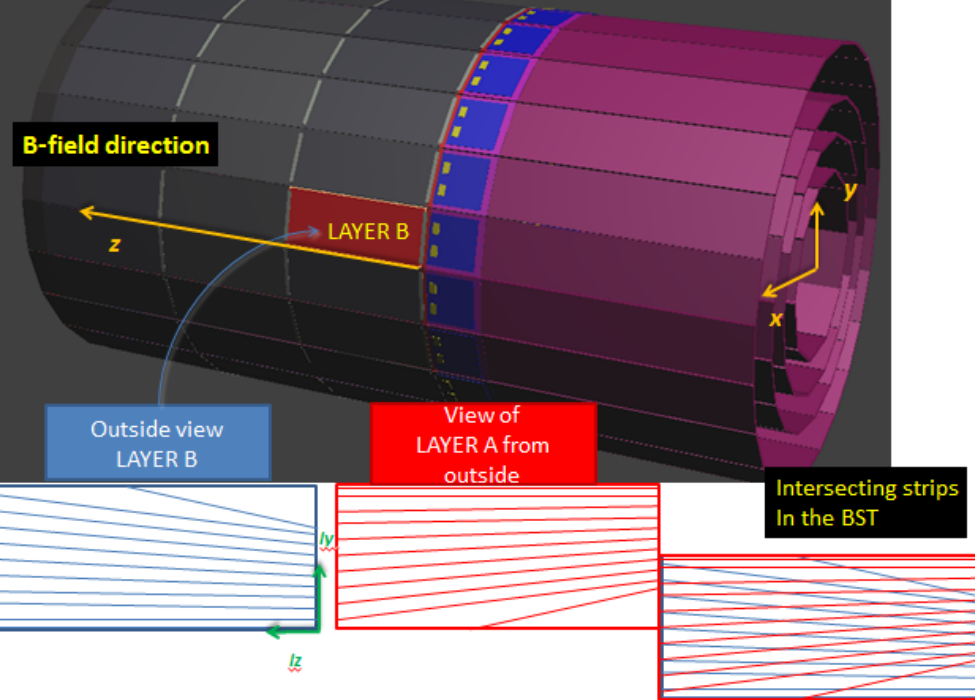
\includegraphics[width=12cm]{Chapters/Ch2-Experiment/clas-12-system/pics/cd/svt.PNG}
    			\caption{Silicon Vertex Tracker}
			\end{figure}  
			
			
			 \begin{figure}[H]
    			\centering
    			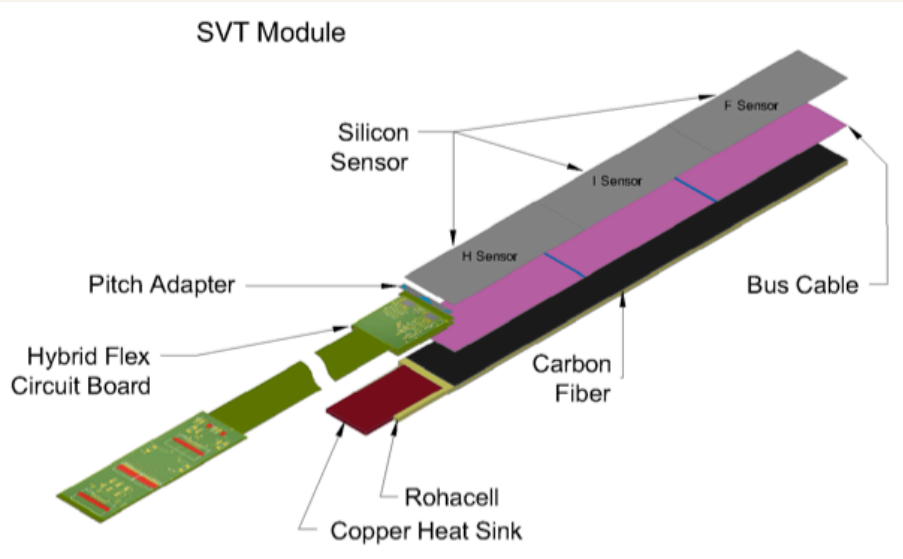
\includegraphics[width=12cm]{Chapters/Ch2-Experiment/clas-12-system/pics/cd/svt-module.PNG}
    			%\caption{SVT Strip}
			\end{figure}  
			
		
		\subsubsection{MMVT}
		    Composed of two parts: a \textbf{Barrel Tracker} and a \textbf{Forward Tracker}. PCB is 200 $\mu$m thick, 0.3\% of a radiation length. 20 MHz sampling frequency. Time resolution of 10 ns. 500 $\mu$m strip pitch.\\
		    \textbf{Advantages of MMVT for CLAS12 :} \\
		    Price: much cheaper compared to SVT. For large area, the price become rapidly prohibitive.
		    Material: Since it is a gasesous detector, it is good for the material budget.
		    Physics Requirements: Not as good spatial resolution as SVT, but can resolve polar angle better. Optimal perform ace is actually achieved with a combination of both detectors are used.
		    \newline
		    Overall momentum uncertainty ($\sigma_p$/p) = 1.6\%. $\sigma_{\theta}$ = 1.4 mrad.  $\sigma_{\phi}$ = 2.6 mrad.  $\sigma _{z}$ = 270 mm.  
		    \subsubsection{Barrel Tracker}
		        18 cylindrical detectors arranged in 6 layers. Covers 35 to 125 degrees. 15,000 readout elements.Gas Mixture 90\% Argon, 10\% isobutane. 3 mm drift gap. 5 kV/cm field. 75\% mesh transparency.
		    \subsubsection{Forward Tracker}
		        6 circular, flat detectors from 6 to 29 degrees in $\theta$. Improves vertex resolution by a factor of up to 10x compared to just the drift chambers along. 6,000 readout elements. 80\% neon, 10\% ethane, 10\% Carbon Tetrafluoride. 5 mm drift gap. 1kV/cm field. 100\% mesh transparency.
		        
		        
		        						
									
			 \begin{figure}[H]
    			\centering
    			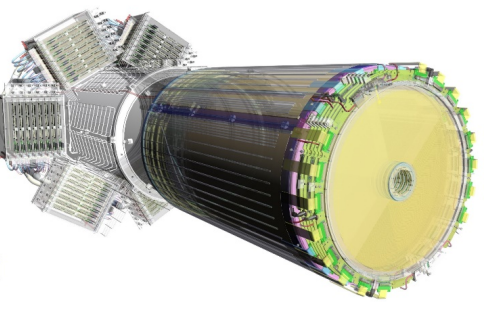
\includegraphics[width=12cm]{Chapters/Ch2-Experiment/clas-12-system/pics/cd/MVT.PNG}
    			%%\caption{SVT Strip}
			\end{figure}
 
    
        \subsubsection{CTOF}
            Central for PID purposes. Divides into 48 1 meter long plastic scintillators with double sided PMT readout.PMTs are in the 0.1 T fringe field region and enclosed in magnetic shielding. 65 picosecond timing resolution. 35 to 125 degrees, 2 $\pi$ in polar angle. 3 cm x 3 cm scintillator planks. Pion/Kaon separation up to 0.64 GeV, Kaon/proton separation up to 1 GeV, pion proton separation up to 1.25 GeV.  
            
            						
			 \begin{figure}[H]
    			\centering
    			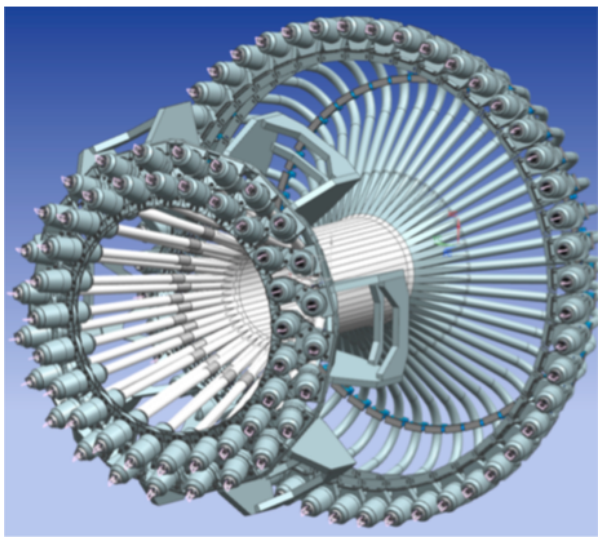
\includegraphics[width=12cm]{Chapters/Ch2-Experiment/clas-12-system/pics/cd/CTOF.PNG}
    			%%\caption{SVT Strip}
			\end{figure}
            
 
		\subsubsection{CND}
		    Detects 0.2-1 GeV neutrons. 3 layers, 48 paddles per layer. Plastic scintillator, 3 cm x 3cm, 0.7 meters  long. Neutron detection efficiency $\sim$ 10\%. 130 picosecond timing resolution, 2 degrees angular resolution (polar and azimuth).
            
            						
			 \begin{figure}[H]
    			\centering
    			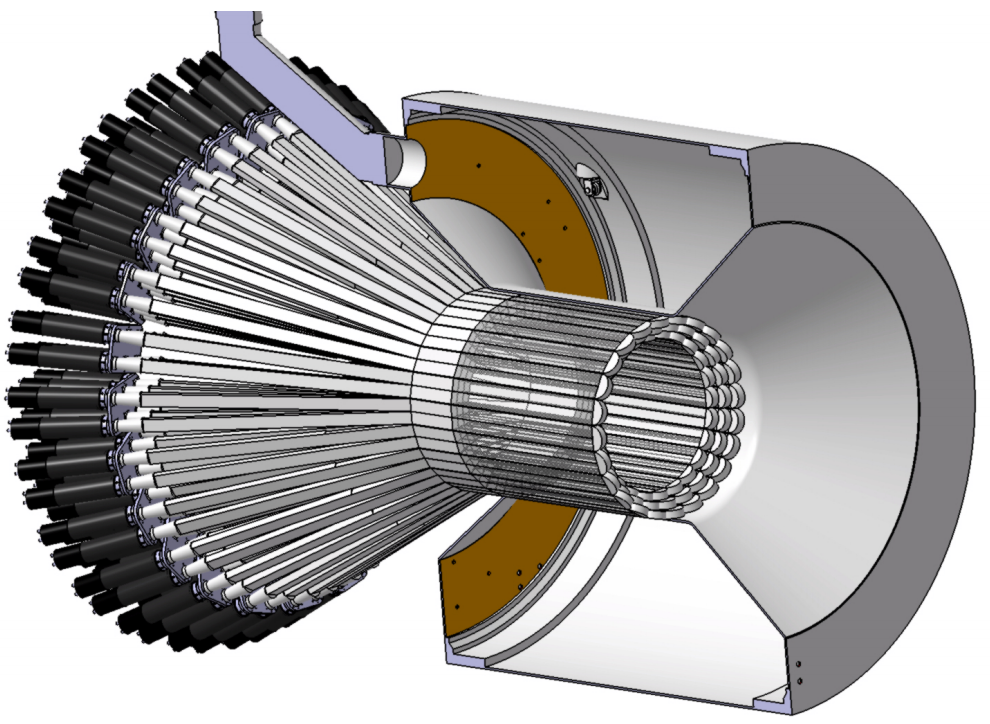
\includegraphics[width=12cm]{Chapters/Ch2-Experiment/clas-12-system/pics/cd/CND.PNG}
    			%%\caption{SVT Strip}
			\end{figure} 

		\subsubsection{Solenoid}
		    5 Tesla super conducting magnet, uniform field ($\Delta$B/B = $10^-4$). Weakest at small angles, strongest at large angles. Opening polar angle of 40 degrees. Momentum range of interest 0.3 to 1.3 GeV. 18 Megajoules stored energy. 85 cm in diameter, 4.2 Kelvin operation. 
		    
    
    \subsubsection{Forward Tagger}
    \subsubsection{BAND}
        BAND not impportant.
    \subsection{Run Conditions}
            CLAS12 runs with "open trigger", which means different sub-experiments can define their own triggering logic. There is a standard electron trigger, based off of hits in HTCC, ECal, and FTOF. 

        Only about 50\% of the electron triggers recorded with an inbending torus polarity are actually electrons. For outbending torus polarity, hte electron trigger purity is as high at 70\%. 
    
    \href{https://www.jlab.org/Hall-B/clas12-web/}{Detector Specs}
    
    20 kHz Level 1 trigger rate, 1 GB/s.


    
    
            \begin{figure}[H]
    			\centering
    			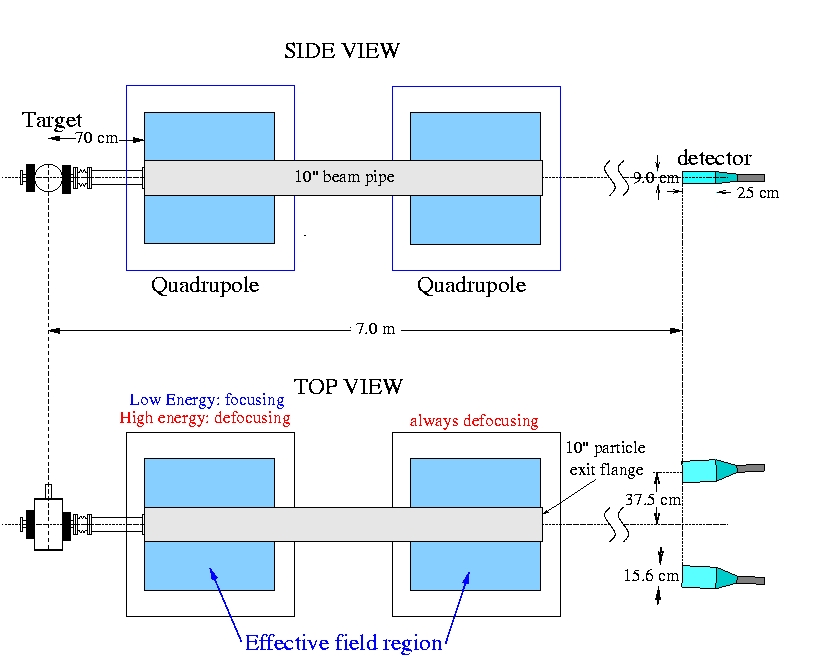
\includegraphics[width=12cm]{Chapters/Ch2-Experiment/clas-12-system/pics/other/hall-b-poll-1.jpg}
    			\caption{ }
			\end{figure}
			
												
			 \begin{figure}[H]
    			\centering
    			\includegraphics[width=12cm]{Chapters/Ch2-Experiment/clas-12-system/pics/other/hall-b-poll-2.jpg}
    			\caption{ }
			\end{figure}
			
			 \begin{figure}[H]
    			\centering
    			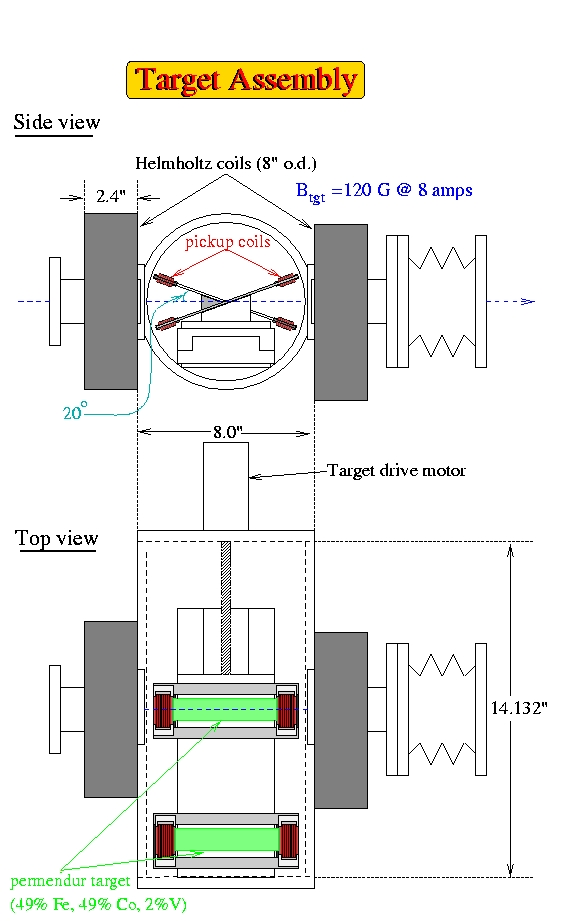
\includegraphics[width=12cm]{Chapters/Ch2-Experiment/clas-12-system/pics/other/hall-b-poll-target.jpg}
    			\caption{ }
			\end{figure}

        Data taken is RGA taken in Fall 2018
    
\section{Reconstruction and Particle Identification}
    here we talk about CLAS PID
\subsection{Decoding and Track Reconstruction}\label{sec:decrec}

\subsection{Particle Identification}


For this analysis all final state particles should be detected.
After $\pi^0$ decay we are going to have 4 particles: electron, proton and two photons.
The particle identification methods are applied to select the exclusive event with at least one electron, proton and two photons. 


    \subsubsection{Electron}
    \subsubsection{Proton}
    \subsubsection{Photon}
    \subsubsection{Pion}
    
    Basic event builder cuts are utilized, then additional cuts are made that are common with the RGA Analysis note (\href{https://www.overleaf.com/project/5ea737720942930001ff5e9c}{overleaf link} and developed by Sangbaek Lee (sangbaek@mit.edu - \href{https://github.com/Sangbaek/analysis_code/tree/analysis/pid}{github code here}. For this analysis, both the central detector and forward detector are utilized for proton tracking. The forward tagger is also utilized for photon identification. 
    


\subsubsection{Neutral pion}
    In addition to individual particle PID procedures the cut on the mass of two photons is applied:
    \begin{itemize}
    	\item $0.07<M_{\gamma\gamma}<0.2$ GeV
    \end{itemize}
    The pion is more thoroughly constrained by the exclusivity cuts, described in the next section.
    

\begin{figure}[hbt]
	\centering
	\includegraphics[page=6,width=0.6\textwidth]{Chapters/Ch4-BaseAnalysis/pid_figs/eppi0.exclusive.pdf}
	
	\caption{The distribution for mass of two photons $M_{\gamma\gamma}$}.
	\label{fig:ggmass}
	
	\centering
	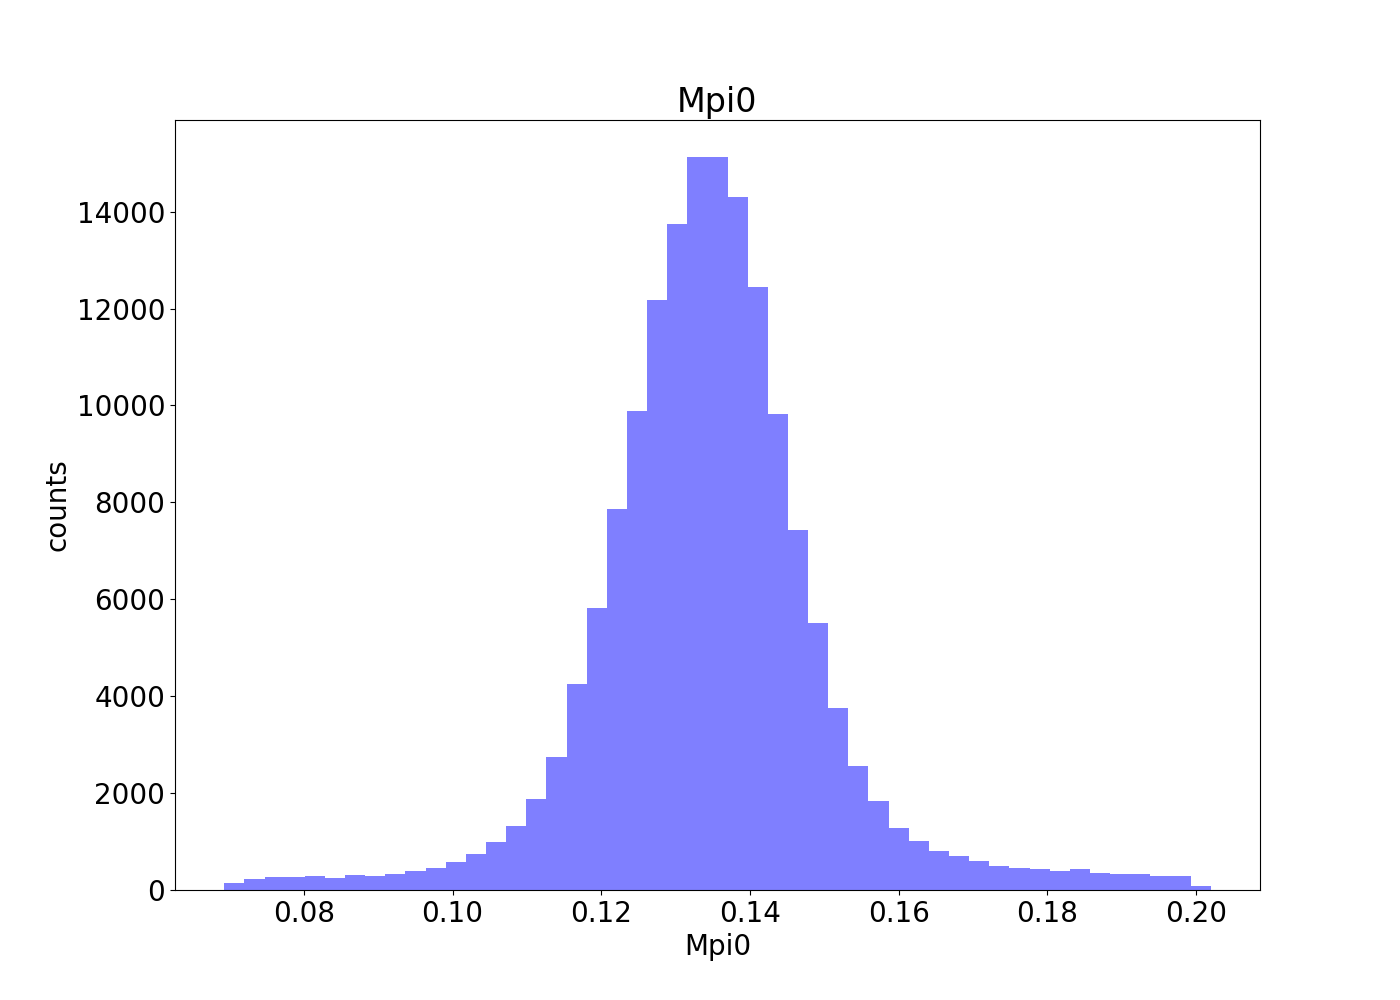
\includegraphics[width=0.6\textwidth]{Chapters/Ch2-Experiment/recon_pid/pid_figs/Mpi0.png}
	
	\caption{The distribution for mass of two photons after exclusivity cuts}.
	\label{fig:ggmass_after}
	
\end{figure}




\subsection{Data Storage and Formatting}
    \subsubsection{Data Location and Availability}
    \subsubsection{File Formatting and Conversion}\label{sec:filtering}
        Mention that same transformations are used for rec events and filtering
    

    






